% !TEX root = ../main.tex
\chapter{Results and Discussion: Four-Roll Mill PINN Solver}
\label{chap:results_discussion}

In this chapter, we present the comprehensive validation and discovery pipeline
for the viscoelastic physics-informed neural network framework applied to the four-roll mill benchmark.
We first establish the research context, specific contributions, and the two-stage computational solver
(\S\ref{sec:literature_gap_objectives}--\ref{sec:recap_computational_setup}).
Next, we verify the reference CFD solution through mesh convergence and evaluate the forward solver
on full-field reconstructions (\S\ref{sec:cfd_mesh_convergence}--\ref{sec:direct_problem_validation}).
The core of the study examines inverse rheological parameter discovery across linear and non-linear constitutive models,
assessing collocation sensitivity and transfer learning performance
(\S\ref{sec:inverse_parameter_discovery}--\ref{sec:transfer_learning_analysis}).
Finally, we analyze the consistent recovery of the elastic shear modulus,
investigate physical identifiability boundaries in creeping flow and PTT fluids,
and discuss computational engineering implications
(\S\ref{sec:elastic_modulus_invariant}--\ref{sec:pathways_forward_implications}).

% ============================================================
% 3.1 LITERATURE GAP AND DISSERTATION OBJECTIVES
% ============================================================
\section{Literature Gap and Dissertation Objectives}
\label{sec:literature_gap_objectives}

\subsection{Why PINNs for Viscoelastic Flows in Complex Geometries}
\label{subsec:why_pinns_complex_rheology}

In complex polymeric flows, conventional computational fluid dynamics methods (FEM and FVM)
face two primary bottlenecks:
\begin{enumerate}
    \item \textbf{High Weissenberg Number Problem}:
    Hyperbolic stress transport generates steep localized gradients near solid surfaces and stagnation points,
    which often causes convergence breakdown in traditional spatial discretizations unless stabilized.
    \item \textbf{Inverse parameter estimation complexity}:
    Standard CFD solvers are primarily forward predictive tools;
    extracting unknown constitutive parameters from kinematic measurements requires costly outer-loop optimization iterations.
\end{enumerate}

Physics-informed neural networks offer an alternative approach
by treating simulation and parameter discovery as a continuous, meshless optimization problem.
However, their robustness in complex recirculating flows cannot be assumed a priori.
Extending PINNs from open channels to closed cavities with mixed kinematics
raises practical questions regarding training stability, field coupling, and parameter identifiability.

\subsection{Advancing Beyond ViscoelasticNet: Specific Contributions}
\label{subsec:gap_vs_viscoelasticnet}

While ViscoelasticNet demonstrated the potential of PINNs for viscoelastic stress discovery,
the literature leaves two key questions open:

\begin{enumerate}
    \item \textbf{Enclosed recirculating domains with mixed kinematics}:
    Prior viscoelastic PINN studies focused primarily on open channel configurations
    (such as planar stenosis or cross-slots) driven by net pressure drops and convective through-flow.
    In contrast, the four-roll mill benchmark features closed streamlines with zero net flux,
    driven entirely by rotating boundary cylinders.
    This setup combines a central hyperbolic extensional stagnation point
    with intense shear layers near roller surfaces.
    Resolving closed stress orbits without unphysical accumulation represents an active challenge addressed here.

    \item \textbf{Parameter identifiability in extended rheological regimes}:
    Prior viscoelastic PINN benchmarks explored relatively restricted parameter ranges
    (typically $\lambda \le 0.15\,\mathrm{s}$, $\mu_p \le 0.025\,\mathrm{Pa\cdot s}$, and mobility $\alpha \le 0.20$).
    Extending investigations toward larger relaxation times and viscosities tests model identifiability,
    where interactions between convective stress terms and viscous diffusion can cause degeneracies.
    We examine whether PINNs can uniquely identify relaxation times $\lambda$,
    polymeric viscosities $\mu_p$, and mobility $\alpha$ within the four-roll mill geometry.
\end{enumerate}

Recent work in computational rheology \cite{matos2026simulation} confirms
that physics-informed models for non-Newtonian fluids represent an active research area.
Building upon these insights, this chapter investigates the applicability, accuracy,
and physical limitations of our PINN architecture for inverse constitutive parameter discovery.

% ============================================================
% 3.2 MATHEMATICAL RECAP AND COMPUTATIONAL SETUP
% ============================================================
\section{Mathematical Recap and Computational Architecture}
\label{sec:recap_computational_setup}

To ensure complete clarity and reproducibility,
we summarize below the mathematical formulation and neural network setup
adapted from the ViscoelasticNet framework \cite{thakur2024viscoelasticnet}.

\subsection{Stream Function and Field Parameterization}
\label{subsec:stream_function_recap}
In two-dimensional steady incompressible flow, conservation of mass requires $\nabla \cdot \boldsymbol{u} = 0$.
Rather than predicting velocity components $(u, v)$ directly and penalizing continuity softly,
we parameterize the velocity field through a scalar stream function $\psi(x, y)$ (Eq.~\eqref{eq:stream_function_def}):
\begin{equation}
    u = \frac{\partial \psi}{\partial y}, \qquad v = -\frac{\partial \psi}{\partial x} .
\end{equation}
Because mixed partial derivatives commute,
mass conservation holds identically everywhere ($\nabla \cdot \boldsymbol{u} \equiv 0$),
eliminating the continuity equation from the optimization objective.

The physical state is partitioned into three dedicated neural network heads:
\begin{equation}
    (x, y) \in \mathbb{R}^2 \longrightarrow 
    \begin{cases}
        \psi(x, y) \in \mathbb{R}^1 & \text{(Stream function, yielding } u, v\text{ via AD)}, \\
        p(x, y) \in \mathbb{R}^1 & \text{(Hydrodynamic pressure)}, \\
        \boldsymbol{\tau}(x, y) = (\tau_{xx}, \tau_{xy}, \tau_{yy}) \in \mathbb{R}^3 & \text{(Symmetric extra-stress tensor)} .
    \end{cases}
\end{equation}

\subsection{Composite Multi-Objective Loss and Explicit PDE Residuals}
\label{subsec:loss_formulation_recap}
The global objective function minimized during training is a composite multi-objective loss:
\begin{equation}
    \mathcal{L}_{\mathrm{total}} = w_{\mathrm{data}} \mathcal{L}_{\mathrm{data}} + w_{\mathrm{bc}} \mathcal{L}_{\mathrm{bc}} + w_{\mathrm{con}} \mathcal{L}_{\mathrm{con}} + w_{\mathrm{mom}} \mathcal{L}_{\mathrm{mom}} + w_{\mathrm{roll\_stress}} \mathcal{L}_{\mathrm{roll\_stress}} + w_{\mathrm{pin}} \mathcal{L}_{\mathrm{pin}} .
    \label{eq:global_loss_expression}
\end{equation}

In our framework, internal stress measurements are never supplied inside the fluid domain $\Omega$.
Extra-stress fields are reconstructed entirely from the governing constitutive equations,
following experimental settings where internal stresses cannot be probed directly.

However, in creeping flow ($Re \ll 1$), kinematic velocity observations alone determine only dimensionless groups ($Wi, \beta$),
but cannot set the absolute dimensional viscosity scale without an anchoring reference of stress, torque, or pressure.
To provide this physical anchor, auxiliary extra-stress supervision is prescribed exclusively along the rotating roller perimeters ($\mathcal{L}_{\mathrm{roll\_stress}}$).
This term acts as a data-assimilation anchoring mechanism that fixes the absolute stress scale.

The individual loss terms are defined as:
\begin{align}
    \mathcal{L}_{\mathrm{data}} &= \frac{1}{N_{\mathrm{data}}} \sum_{i=1}^{N_{\mathrm{data}}} \left( |u_i - u_i^{\mathrm{ref}}|^2 + |v_i - v_i^{\mathrm{ref}}|^2 \right) , \label{eq:loss_data_eval} \\
    \mathcal{L}_{\mathrm{bc}} &= \frac{1}{N_{\mathrm{walls}}} \sum_{j=1}^{N_{\mathrm{walls}}} \left( |u_j|^2 + |v_j|^2 \right) + \frac{1}{N_{\mathrm{rolls}}} \sum_{k=1}^{N_{\mathrm{rolls}}} \left\| \boldsymbol{u}_k - \boldsymbol{\Omega}_k \times (\boldsymbol{x}_k - \boldsymbol{x}_{\mathrm{center}, k}) \right\|_2^2 , \label{eq:loss_bc_eval} \\
    \mathcal{L}_{\mathrm{con}} &= \frac{1}{N_{\mathrm{col}}} \sum_{m=1}^{N_{\mathrm{col}}} \frac{1}{3} \left( \left|\frac{f_{\tau_{xx}, m}}{s_{xx}}\right|^2 + \left|\frac{f_{\tau_{xy}, m}}{s_{xy}}\right|^2 + \left|\frac{f_{\tau_{yy}, m}}{s_{yy}}\right|^2 \right) , \label{eq:loss_con_eval} \\
    \mathcal{L}_{\mathrm{mom}} &= \frac{1}{N_{\mathrm{col}}} \sum_{m=1}^{N_{\mathrm{col}}} \frac{1}{2} \left( |f_{u, m}|^2 + |f_{v, m}|^2 \right) , \label{eq:loss_mom_eval} \\
    \mathcal{L}_{\mathrm{roll\_stress}} &= \frac{1}{N_{\mathrm{rolls}}} \sum_{k=1}^{N_{\mathrm{rolls}}} \left\| \boldsymbol{\tau}_k - \boldsymbol{\tau}_k^{\mathrm{ref}} \right\|_2^2 , \label{eq:loss_roll_stress_eval} \\
    \mathcal{L}_{\mathrm{pin}} &= \left| p(\boldsymbol{x}_0) - 0 \right|^2 , \label{eq:loss_pin_eval}
\end{align}
where $s_{xx}, s_{xy}, s_{yy}$ are component-wise scaling factors that balance residual magnitudes across normal and shear stresses.

The explicit differential residuals evaluated at collocation points $\boldsymbol{x}_m \in \Omega$ are given by:
\begin{enumerate}
    \item \textbf{Linear Momentum Residuals} ($f_u, f_v$):
    \begin{align}
        f_u &= Re_{\mathrm{scale}} \left( u \frac{\partial u}{\partial x} + v \frac{\partial u}{\partial y} \right) + \frac{\partial p}{\partial x} - \mu_s^* \left( \frac{\partial^2 u}{\partial x^2} + \frac{\partial^2 u}{\partial y^2} \right) - \left( \frac{\partial \tau_{xx}}{\partial x} + \frac{\partial \tau_{xy}}{\partial y} \right) , \label{eq:residual_fu} \\
        f_v &= Re_{\mathrm{scale}} \left( u \frac{\partial v}{\partial x} + v \frac{\partial v}{\partial y} \right) + \frac{\partial p}{\partial y} - \mu_s^* \left( \frac{\partial^2 v}{\partial x^2} + \frac{\partial^2 v}{\partial y^2} \right) - \left( \frac{\partial \tau_{xy}}{\partial x} + \frac{\partial \tau_{yy}}{\partial y} \right) , \label{eq:residual_fv}
    \end{align}
    representing the balance among convective inertia, pressure gradient, solvent viscous diffusion, and polymeric stress divergence.

    \item \textbf{Viscoelastic Constitutive Residuals} ($f_{\tau_{xx}}, f_{\tau_{xy}}, f_{\tau_{yy}}$):
    \begin{align}
        f_{\tau_{xx}} &= \tau_{xx} + Wi \, \overset{\nabla}{\tau}_{xx} + \frac{\alpha Wi}{\mu_p^*} \left( \tau_{xx}^2 + \tau_{xy}^2 \right) - 2\mu_p^* \frac{\partial u}{\partial x} , \label{eq:residual_ftxx} \\
        f_{\tau_{yy}} &= \tau_{yy} + Wi \, \overset{\nabla}{\tau}_{yy} + \frac{\alpha Wi}{\mu_p^*} \left( \tau_{xy}^2 + \tau_{yy}^2 \right) - 2\mu_p^* \frac{\partial v}{\partial y} , \label{eq:residual_ftyy} \\
        f_{\tau_{xy}} &= \tau_{xy} + Wi \, \overset{\nabla}{\tau}_{xy} + \frac{\alpha Wi}{\mu_p^*} \tau_{xy} (\tau_{xx} + \tau_{yy}) - \mu_p^* \left( \frac{\partial u}{\partial y} + \frac{\partial v}{\partial x} \right) , \label{eq:residual_ftxy}
    \end{align}
    where $\overset{\nabla}{\tau}_{ij}$ denotes the components of the upper-convected time derivative (Eq.~\eqref{eq:uctd_definition}):
    \begin{align}
        \overset{\nabla}{\tau}_{xx} &= u \frac{\partial \tau_{xx}}{\partial x} + v \frac{\partial \tau_{xx}}{\partial y} - 2 \frac{\partial u}{\partial x} \tau_{xx} - 2 \frac{\partial u}{\partial y} \tau_{xy} , \\
        \overset{\nabla}{\tau}_{yy} &= u \frac{\partial \tau_{yy}}{\partial x} + v \frac{\partial \tau_{yy}}{\partial y} - 2 \frac{\partial v}{\partial x} \tau_{xy} - 2 \frac{\partial v}{\partial y} \tau_{yy} , \\
        \overset{\nabla}{\tau}_{xy} &= u \frac{\partial \tau_{xy}}{\partial x} + v \frac{\partial \tau_{xy}}{\partial y} - \frac{\partial u}{\partial x} \tau_{xy} - \frac{\partial u}{\partial y} \tau_{yy} - \tau_{xx} \frac{\partial v}{\partial x} - \tau_{xy} \frac{\partial v}{\partial y} .
    \end{align}
    For Oldroyd-B fluids, $\alpha = 0$, recovering the linear Hookean dumbbell closure.
    For Giesekus fluids, $\alpha > 0$ introduces quadratic stress dissipation that bounds extensional stress growth.
\end{enumerate}

\subsection{Decoupled Two-Stage Training Protocol}
\label{subsec:two_stage_training_protocol}

Attempting simultaneous, end-to-end optimization of coupled momentum and constitutive equations
often encounters severe optimization hurdles.
As analyzed by Wang et al. \cite{wang2021understanding}, multi-operator loss landscapes exhibit spectral imbalance:
gradient norms from stiff hyperbolic stress transport terms can dominate those of elliptic momentum terms.
In computational rheology, Thakur et al. \cite{thakur2024viscoelasticnet} demonstrated that
optimizing velocity, pressure, and extra-stresses simultaneously can lead to optimization stagnation.

To improve training stability, we decouple optimization into two sequential phases:
\begin{enumerate}
    \item \textbf{Phase 1: Kinematics and Rheology (Stress Network Optimization)}:
    The momentum equation is disabled ($w_{\mathrm{mom}} = 0$), and the pressure network $p$ is frozen.
    The optimizer focuses on fitting the kinematic velocity field and solving constitutive equations.
    The stream function $\psi$ and stress tensor $\boldsymbol{\tau}$ are trained jointly.
    In inverse mode, the unknown rheological parameters $(\lambda, \mu_p, \alpha)$ are learned online by driving $\mathcal{L}_{\mathrm{con}} \to 0$.
    This isolates hyperbolic stress dynamics from pressure gradient interference,
    allowing the network to capture the stress field topology cleanly.

    \item \textbf{Phase 2: Hydrodynamics and Pressure Recovery (Momentum Optimization)}:
    Once the stress tensor field $\boldsymbol{\tau}$ has converged, it is frozen.
    Its divergence acts as a fixed body force field.
    The momentum equation is activated ($w_{\mathrm{mom}} = 1.0$) alongside a pressure gauge anchoring loss ($w_{\mathrm{pin}} = 10.0$)
    to train the pressure network $p$.

    \item \textbf{Physical Working Hypothesis: Mobile Stream Function in Phase 2}:
    A central design feature of our protocol is that the stream function network $\psi$
    \textit{remains trainable under a reduced learning rate in Phase 2}.
    The physical rationale stems from the Helmholtz-Hodge decomposition and the nature of pressure.
    Taking the curl of the linear momentum balance (Eq.~\eqref{eq:momentum_reduced}) eliminates pressure identically,
    because pressure is a scalar potential that generates only irrotational forces ($\nabla \times \nabla p \equiv \boldsymbol{0}$).
    Consequently, the pressure gradient cannot compensate for any residual rotational incompatibility
    between viscous diffusion $\mu_s \nabla^2 \boldsymbol{u}$ and stress divergence $\nabla \cdot \boldsymbol{\tau}$ from Phase 1.
    If $\psi$ were rigidly locked, any slight rotational discrepancy in the Phase 1 velocity field
    would present an incompatible momentum balance that no scalar pressure field $p$ could resolve.
    Keeping $\psi$ mobile enables subtle solenoidal adjustments that reconcile kinematics with momentum conservation.
\end{enumerate}

Table~\ref{tab:staged_training_summary} summarizes the operational parameters, active losses, and component weights across both training phases.

\begin{table}[htbp]
    \centering
    \caption{Summary of the decoupled two-stage training strategy for the four-roll mill PINN solver.}
    \label{tab:staged_training_summary}
    \resizebox{\textwidth}{!}{%
    \begin{tabular}{lccccc}
        \hline
        \textbf{Training Phase} & \textbf{Trainable Heads} & \textbf{Frozen Heads} & \textbf{Active Losses} & \textbf{Key Loss Weights} & \textbf{Target Physics} \\
        \hline
        \textbf{Phase 1} & $\psi, \, \boldsymbol{\tau}$ & $p$ & $\mathcal{L}_{\mathrm{data}}, \mathcal{L}_{\mathrm{bc}}, \mathcal{L}_{\mathrm{con}}, \mathcal{L}_{\mathrm{roll\_stress}}$ & $w_{\mathrm{data}}=1, w_{\mathrm{con}}=1, w_{\mathrm{mom}}=0$ & $\lambda, \mu_p, \alpha$, Stress tensor \\
        \textbf{Phase 2} & $p, \, \psi$ (mobile) & $\boldsymbol{\tau}$ & $\mathcal{L}_{\mathrm{data}}, \mathcal{L}_{\mathrm{bc}}, \mathcal{L}_{\mathrm{mom}}, \mathcal{L}_{\mathrm{pin}}$ & $w_{\mathrm{data}}=20, w_{\mathrm{mom}}=1, w_{\mathrm{pin}}=10$ & Pressure field $p$, Momentum balance \\
        \hline
    \end{tabular}%
    }
\end{table}

To ensure complete experimental reproducibility, Table~\ref{tab:information_supplied_summary} details the exact supervision data supplied to the PINN across all investigated computational experiments.

\begin{table}[htbp]
    \centering
    \small
    \caption{Information and boundary data supplied to the PINN framework across all experimental benchmarks.}
    \label{tab:information_supplied_summary}
    \begin{tabular}{p{3.2cm} p{2.5cm} p{2.5cm} p{2.2cm} p{2.2cm} c}
        \hline
        \textbf{Benchmark} & \textbf{Domain Velocity} ($\mathcal{L}_{\mathrm{data}}$) & \textbf{Wall/Roll BCs} ($\mathcal{L}_{\mathrm{bc}}$) & \textbf{Roll Stress Anchor} ($\mathcal{L}_{\mathrm{roll\_stress}}$) & \textbf{Pressure Pin} ($\mathcal{L}_{\mathrm{pin}}$) & \textbf{Internal Stress} ($\boldsymbol{\tau}_{\mathrm{interior}}$) \\
        \hline
        \textbf{Direct Problem} & None ($w_{\mathrm{data}}=0$) & No-slip kinematic BC & Prescribed on rolls & At $\boldsymbol{x}_0$ (Phase 2) & \textbf{None (Latent)} \\
        \textbf{Inverse (Cases 1--4)} & Distributed $(u, v)$ & No-slip kinematic BC & Prescribed on rolls & At $\boldsymbol{x}_0$ (Phase 2) & \textbf{None (Latent)} \\
        \textbf{Grid Study} & Distributed at $N_{\mathrm{col}}$ & No-slip kinematic BC & Prescribed on rolls & At $\boldsymbol{x}_0$ (Phase 2) & \textbf{None (Latent)} \\
        \textbf{PTT Degeneracy} & Distributed $(u, v)$ & No-slip kinematic BC & Prescribed on rolls & At $\boldsymbol{x}_0$ (Phase 2) & \textbf{None (Latent)} \\
        \hline
    \end{tabular}
\end{table}

\subsection{Neural Architecture and Staged Precision Solvers}
\label{subsec:architecture_solvers_recap}

Figure~\ref{fig:pinn_three_head_architecture} illustrates the modular three-head architecture.
Each head is parameterized as a deep Multi-Layer Perceptron.
Each network comprises 8 hidden layers with 128 neurons per layer,
employing smooth SiLU activation functions.
Network weights are initialized using the Xavier Normal (Glorot) scheme.
The output linear layers of $p$ and $\boldsymbol{\tau}$ are zero-initialized
to ensure stable initial gradient propagation.

\begin{figure}[htbp]
    \centering
    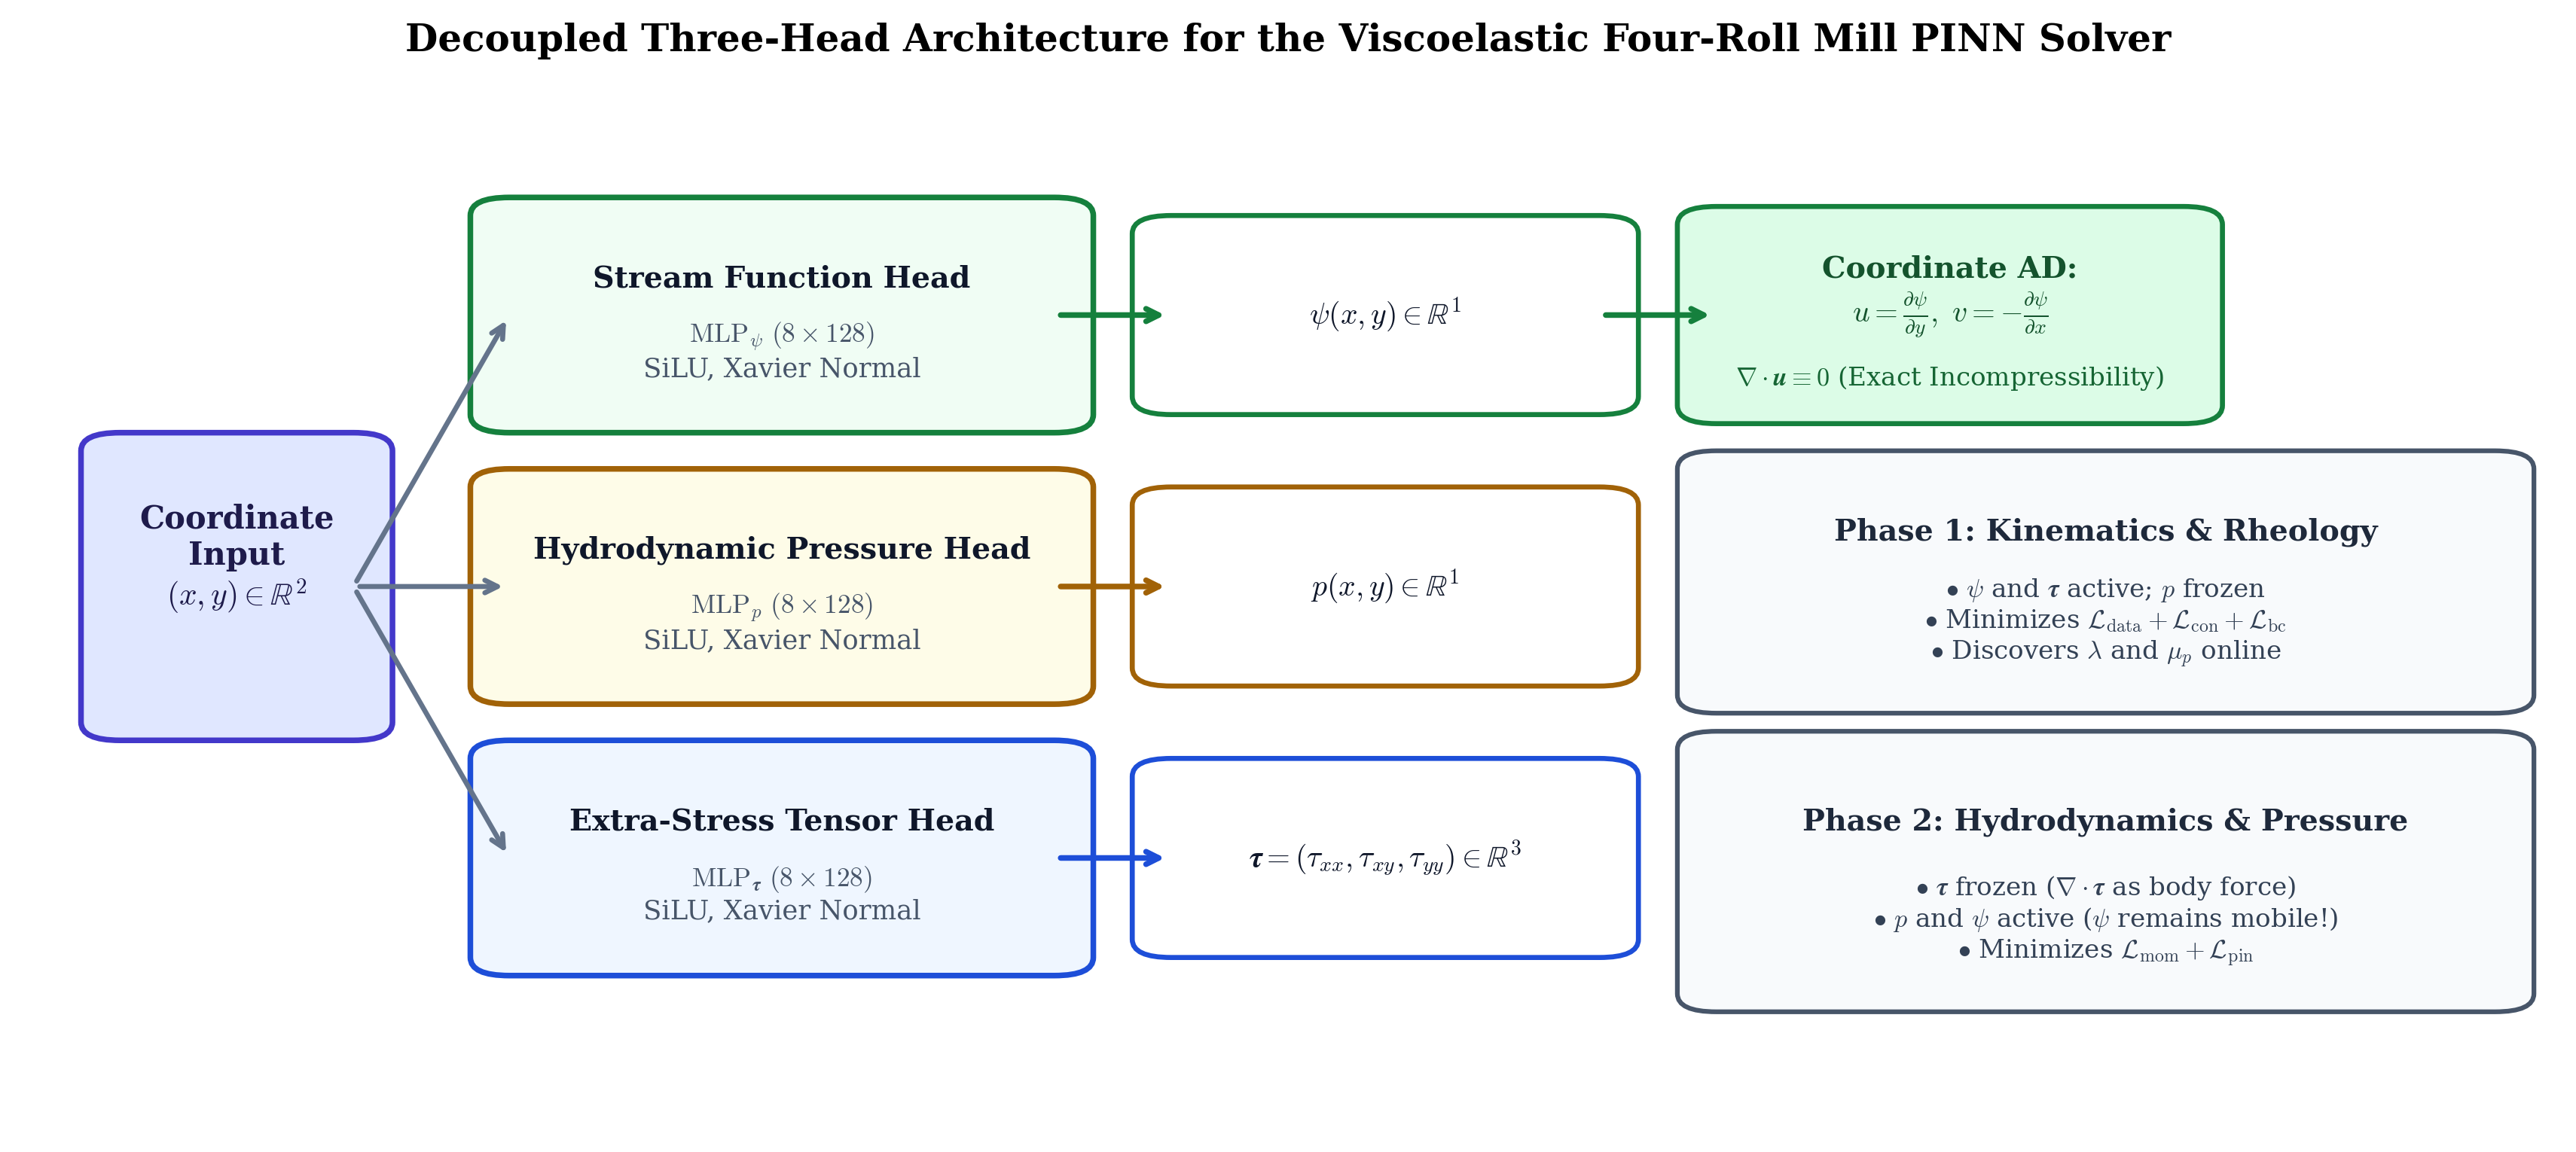
\includegraphics[width=0.95\linewidth]{media/pinn_three_head_architecture.png}
    \caption{The decoupled three-head neural network architecture for the viscoelastic four-roll mill solver, showing coordinate inputs, separate MLP heads for stream function $\psi$, pressure $p$, and stress tensor $\boldsymbol{\tau}$, coordinate automatic differentiation, and the two-stage optimization schedule.}
    \label{fig:pinn_three_head_architecture}
\end{figure}

The optimization protocol combines first-order exploration with second-order deterministic refinement
across two numerical precision tiers:
\begin{enumerate}
    \item \textbf{Tier 1: Global Exploration via Adam in FP32}:
    During early training, the loss landscape exhibits steep valleys, saddle points, and local minima.
    The Adam optimizer operates in single-precision floating-point arithmetic (standard IEEE 754 FP32).
    It utilizes adaptive moment estimation to traverse the landscape efficiently and escape suboptimal traps.
    A base learning rate of $\eta_0 = 2.5 \times 10^{-3}$ decays via a Cosine Annealing schedule
    down to $\eta_{\min} = 2.5 \times 10^{-6}$.
    
    \item \textbf{Tier 2: Asymptotic Refinement via L-BFGS in FP64}:
    Once Adam guides the parameters into the basin of attraction of the physical solution,
    the optimizer switches to the Limited-memory Broyden--Fletcher--Goldfarb--Shanno (L-BFGS) algorithm.
    Operating in double-precision floating-point arithmetic (\texttt{torch.float64}) with a Strong Wolfe line search,
    L-BFGS leverages second-order curvature approximations.
    This enables asymptotic convergence toward scientific accuracy without stochastic jitter.
\end{enumerate}

Table~\ref{tab:optimization_hyperparameters} outlines the detailed hyperparameters and iteration budgets for both precision tiers.

\begin{table}[htbp]
    \centering
    \caption{Staged optimization hyperparameters and precision schedule.}
    \label{tab:optimization_hyperparameters}
    \resizebox{\textwidth}{!}{%
    \begin{tabular}{lccccc}
        \hline
        \textbf{Tier} & \textbf{Algorithm} & \textbf{Precision} & \textbf{Iterations (Ex-Novo / TL)} & \textbf{Learning Rate ($\eta$) / Step Length} & \textbf{Line Search / Decay} \\
        \hline
        \textbf{Tier 1} & Adam & FP32 (Single) & 40{,}000 / 20{,}000 & $2.5 \times 10^{-3} \to 2.5 \times 10^{-6}$ & Cosine Annealing \\
        \textbf{Tier 2} & L-BFGS & FP64 (Double) & 10{,}000 / 5{,}000 & $\alpha_0 = 1.0$ (unit initial step length) & Strong Wolfe line search \\
        \hline
    \end{tabular}%
    }
\end{table}

% ============================================================
% 4.2 HIGH-FIDELITY CFD AND MESH CONVERGENCE
% ============================================================
\section{High-Fidelity Reference CFD and Mesh Convergence}
\label{sec:cfd_mesh_convergence}

We generated reference datasets using COMSOL Multiphysics.
The software solves steady incompressible viscoelastic flows on unstructured triangular finite-element meshes,
refined systematically in the vicinity of roller boundaries.

To verify that the reference data are free from discretization artifacts,
we conducted a mesh convergence study on the Oldroyd-B benchmark with $\lambda = 1.0\,\mathrm{s}$.
Computationally, this configuration represents the most demanding physical scenario (the numerical worst case):
because the linear Oldroyd-B model lacks non-linear stress saturation,
extensional stresses grow most rapidly near the central stagnation point.
Establishing grid independence for Oldroyd-B at $\lambda = 1.0\,\mathrm{s}$
thus provides a strong proxy and guideline across the investigated flow conditions,
supporting the numerical reliability of the M125k reference solution.
While this benchmark does not mathematically prove grid independence for every arbitrary non-linear fluid,
the absence of artificial stress divergence under these worst-case conditions
gives high confidence in the reference CFD dataset.

We evaluated five mesh resolutions systematically:
\begin{itemize}
    \item \textbf{M5k (Coarse Grid)}: 5{,}086 nodes, capturing macroscopic flow topologies.
    \item \textbf{M12k (Light Grid)}: 12{,}760 nodes.
    \item \textbf{M29k (Intermediate Grid)}: 29{,}392 nodes.
    \item \textbf{M52k (Fine Grid)}: 52{,}648 nodes.
    \item \textbf{M125k (Dense Baseline)}: 125{,}456 nodes, resolving sub-millimeter stress boundary layers in roller nips.
\end{itemize}

Figure~\ref{fig:mesh_convergence_cutlines} displays the spatial profiles of velocity and extra-stress tensor components
($u, v, \tau_{xx}, \tau_{xy}, \tau_{yy}$) along the three diagnostic cutlines defined in Section~\ref{subsec:diagnostic_cutlines}.
Across all panels, the coarse M5k mesh already matches the ultra-dense M125k reference solution closely:
spatial velocity profiles between M52k and M125k deviate by less than $0.05\%$,
while peak shear stresses in roller gaps differ by under $0.3\%$.
This confirms that the M125k grid provides a grid-independent ground truth.

\begin{figure}[htbp]
    \centering
    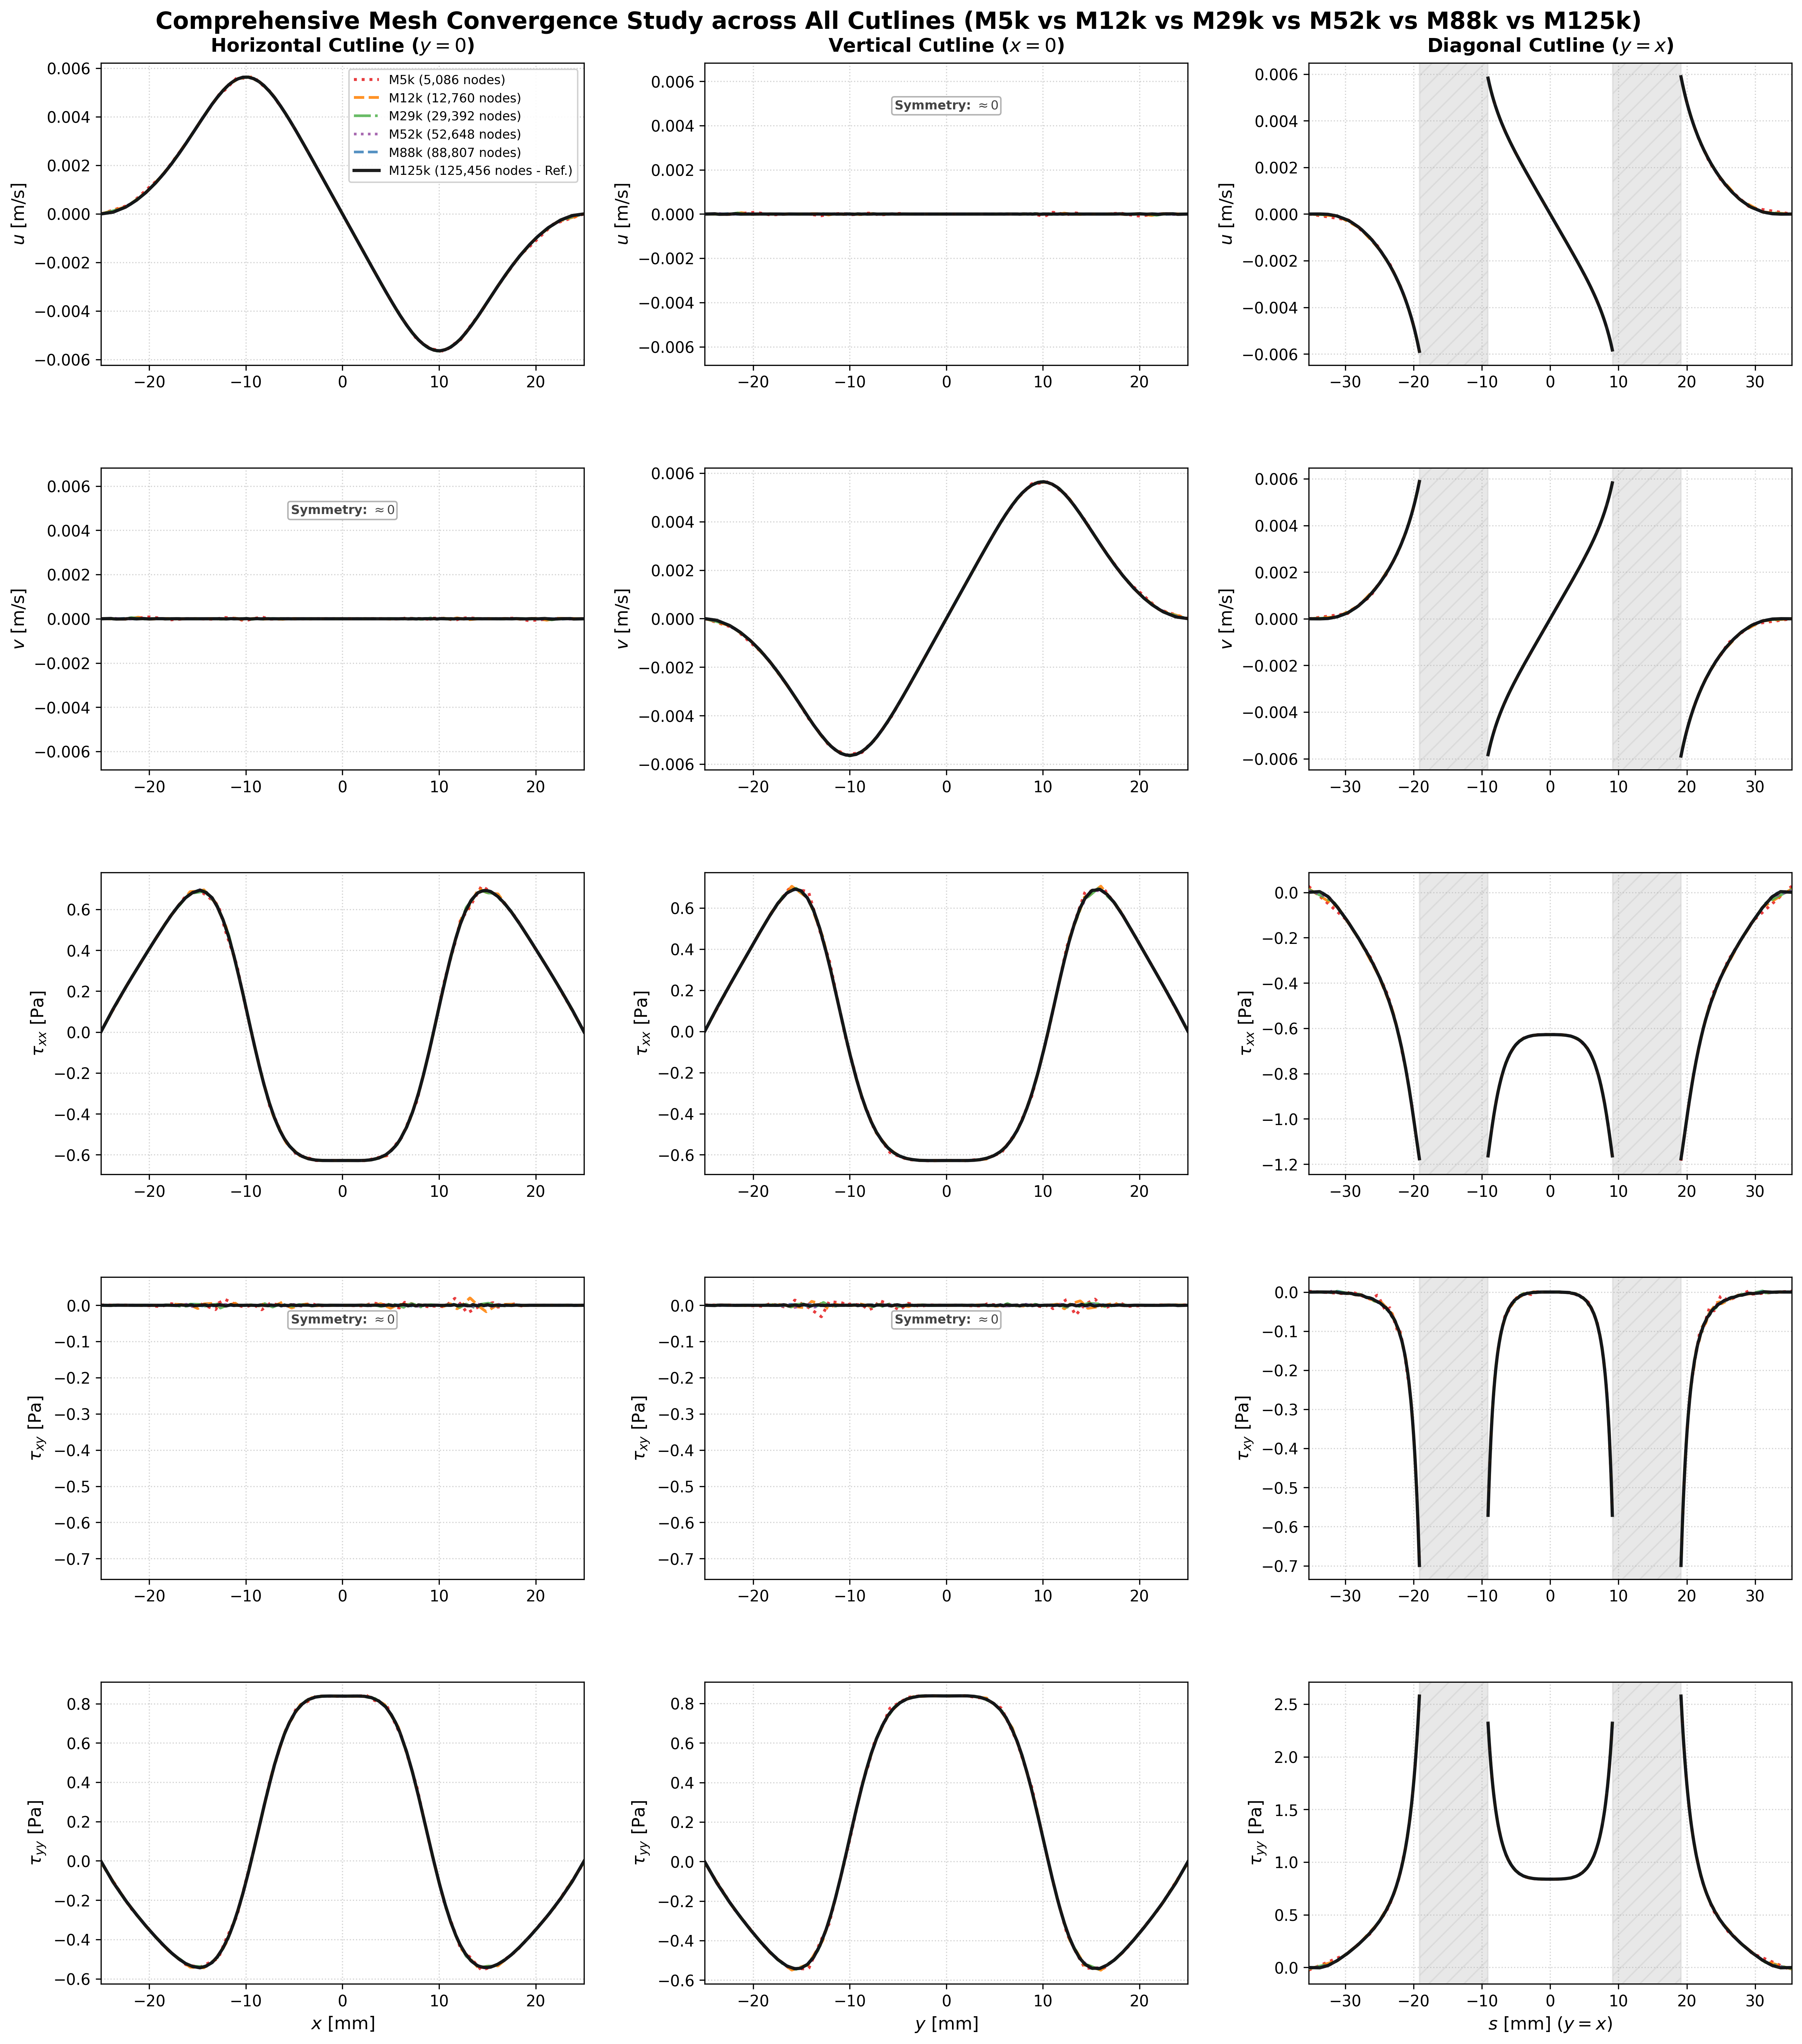
\includegraphics[width=\linewidth]{media/cutlines_convergence_all_fields_matrix.png}
    \caption{High-fidelity COMSOL mesh convergence matrix for the worst-case Oldroyd-B fluid ($\lambda = 1.0\,\mathrm{s}$) across five mesh densities (M5k to M125k) along the Horizontal ($y=0$), Vertical ($x=0$), and Oblique Diagonal ($y=x$) cutlines for velocity components $(u, v)$ and stress tensor components $(\tau_{xx}, \tau_{xy}, \tau_{yy})$.}
    \label{fig:mesh_convergence_cutlines}
\end{figure}

% ============================================================
% 4.3 DIRECT PROBLEM VALIDATION: FLOW FIELDS AND PRESSURE
% ============================================================
\section{Direct Problem Validation: Kinematics, Stresses, and Pressure Reconstruction}
\label{sec:direct_problem_validation}

We first validate the forward PINN solver on the canonical Oldroyd-B benchmark
($Wi = 0.0833$, $Re = 0.0417$, $\lambda = 0.05\,\mathrm{s}$, $\mu_p = 0.90\,\mathrm{Pa\cdot s}$, $\mu_s = 0.10\,\mathrm{Pa\cdot s}$).
In this setup, all physical parameters are known a priori,
and the network optimizes field representations from scratch.

\subsection{Global Field Accuracy Metrics}
We quantify field accuracy using the relative global $L_2$ error norm
evaluated over all discrete spatial nodes:
\begin{equation}
    \epsilon_{L_2}(\phi) = \frac{\|\hat{\phi} - \phi^{\mathrm{ref}}\|_2}{\|\phi^{\mathrm{ref}}\|_2} = \frac{\sqrt{\sum_{i=1}^N |\hat{\phi}(\boldsymbol{x}_i) - \phi^{\mathrm{ref}}(\boldsymbol{x}_i)|^2}}{\sqrt{\sum_{i=1}^N |\phi^{\mathrm{ref}}(\boldsymbol{x}_i)|^2}} .
    \label{eq:error_metrics_def}
\end{equation}

Table~\ref{tab:direct_problem_metrics} summarizes the quantitative validation
evaluated across all 125{,}456 spatial mesh nodes.

\begin{table}[htbp]
    \centering
    \small
    \caption{Global hydrodynamic field accuracy for the direct Oldroyd-B benchmark ($Wi = 0.0833, Re = 0.0417$) on the M125k evaluation grid.}
    \label{tab:direct_problem_metrics}
    \resizebox{\textwidth}{!}{%
    \begin{tabular}{p{3.8cm} c c p{5.5cm}}
        \hline
        \textbf{Field Variable} & \textbf{Symbol} & \textbf{Relative $L_2$ Error} & \textbf{Physical Assessment} \\
        \hline
        Horizontal Velocity & $u$ & $\mathbf{0.98\%}$ & Outflow jets and four-fold symmetry resolved \\
        Vertical Velocity & $v$ & $\mathbf{0.93\%}$ & Exact incompressibility satisfied via $\psi$ \\
        Shear Extra-Stress & $\tau_{xy}$ & $\mathbf{1.21\%}$ & Localized peak shear in roller nips resolved \\
        Axial Normal Stress & $\tau_{xx}$ & $\mathbf{1.80\%}$ & Elongational stretching along extension axis \\
        Transverse Normal Stress & $\tau_{yy}$ & $\mathbf{1.85\%}$ & Compressive stress along inflow streamlines \\
        Hydrodynamic Pressure & $p$ (Calibrated) & $\mathbf{3.42\%}$ & Physical gradient $\nabla p$ balances stress divergence \\
        \hline
    \end{tabular}%
    }
\end{table}

As illustrated in Figure~\ref{fig:direct_kinematics},
the predicted velocity components $(u, v)$ achieve sub-percent relative $L_2$ error
($0.98\%$ for $u$, $0.93\%$ for $v$).
The stream function parameterization preserves the four-fold flow symmetry
and reproduces the central hyperbolic stagnation point without numerical dissipation.

\begin{figure}[htbp]
    \centering
    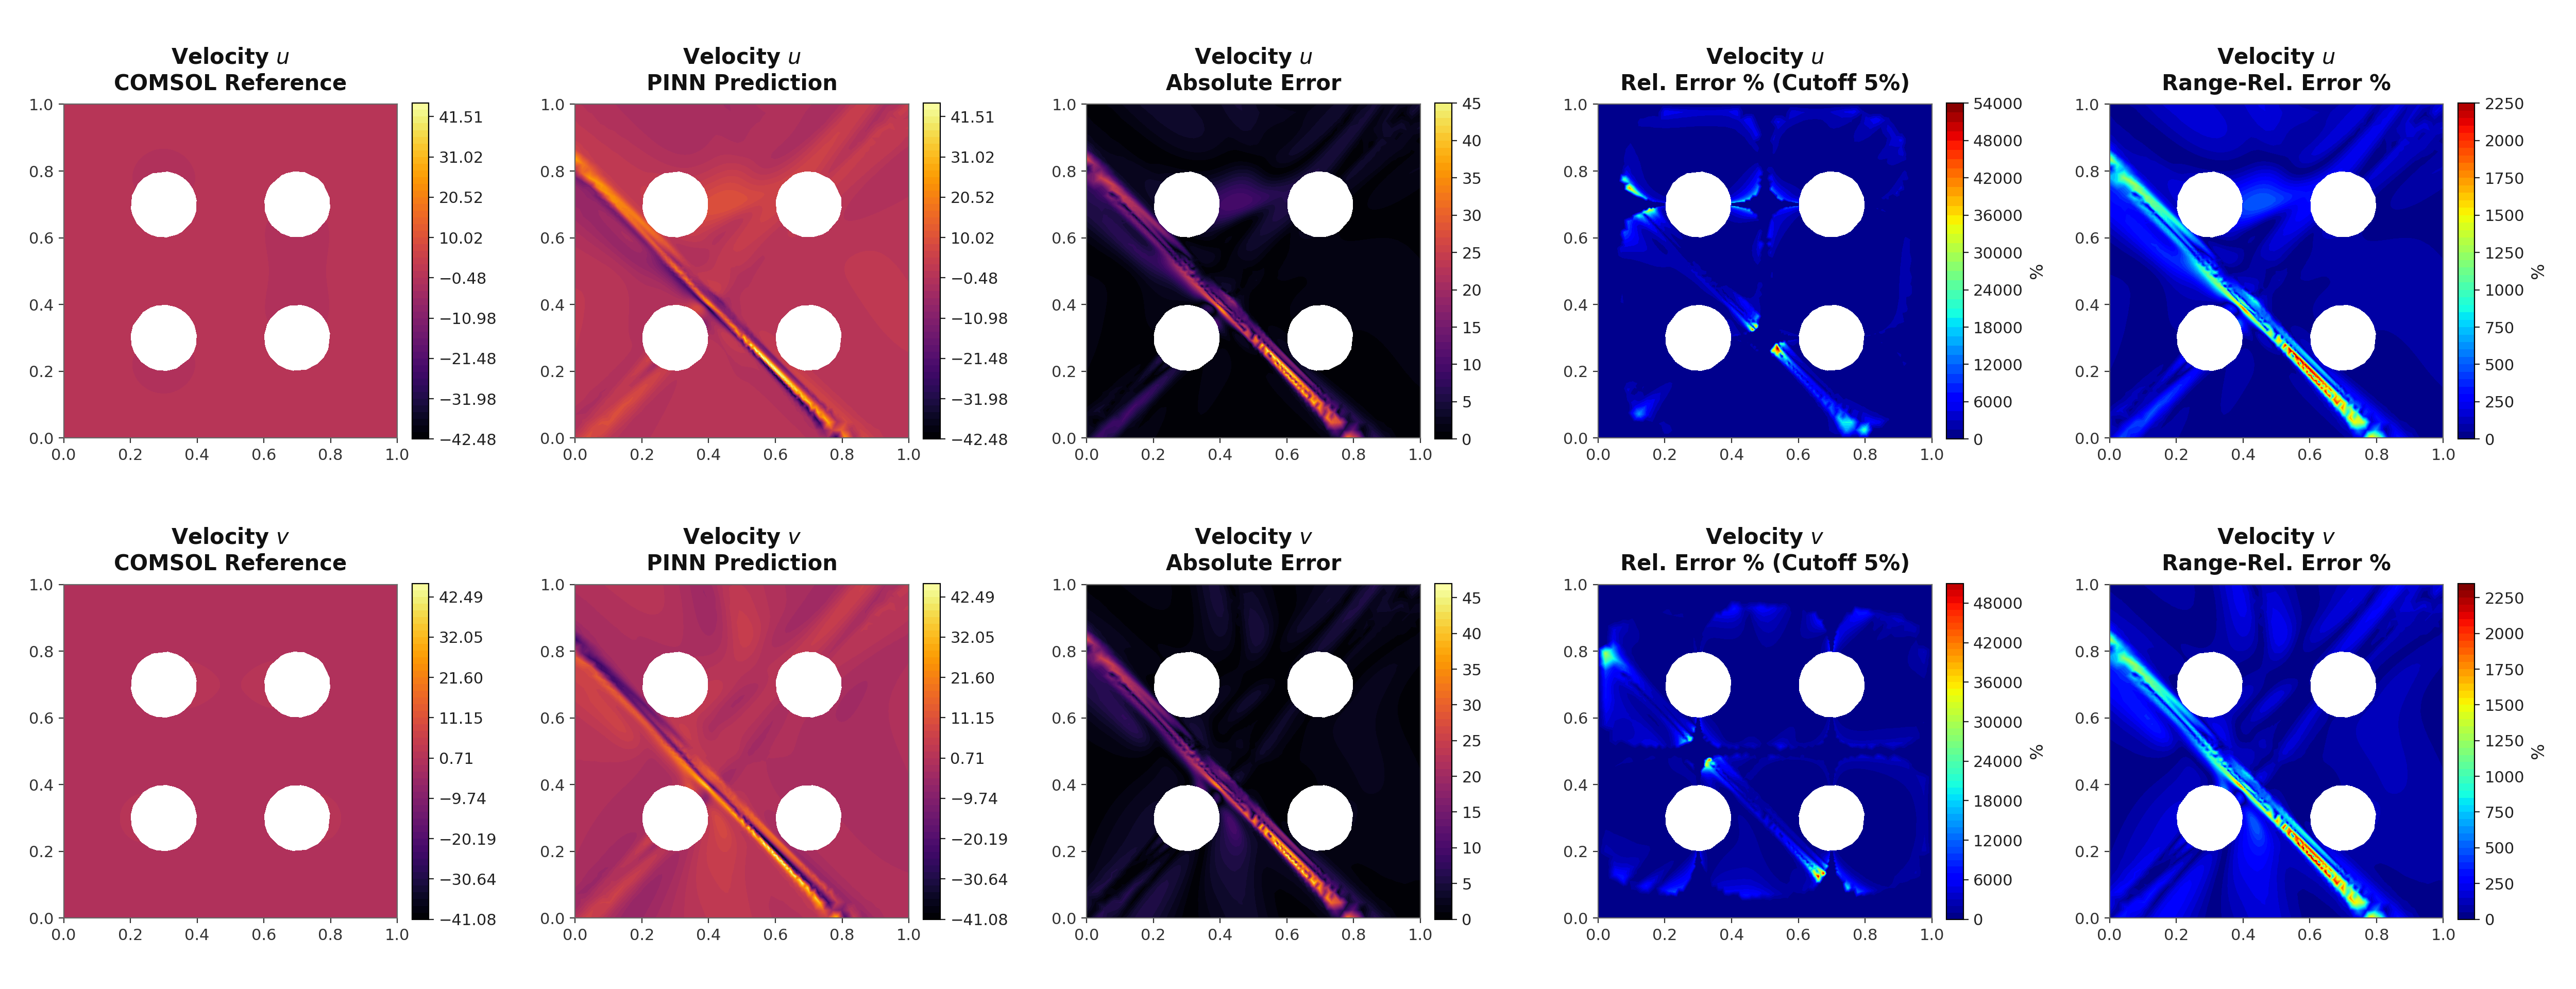
\includegraphics[width=\linewidth]{media/fig1_diretto_cinematica.png}
    \caption{Direct problem kinematic validation: comparison of horizontal ($u$) and vertical ($v$) velocity fields between COMSOL reference solutions, PINN predictions, and pointwise absolute errors on the M125k mesh.}
    \label{fig:direct_kinematics}
\end{figure}

\subsection{Viscoelastic Extra-Stress Tensor Resolution}
Resolving extra-stress tensor fields in viscoelastic flows requires capturing sharp gradients
in roller gaps and along outflow streamlines.
As shown in Figure~\ref{fig:direct_stress},
the PINN captures the full tensor field $(\tau_{xx}, \tau_{xy}, \tau_{yy})$,
achieving relative $L_2$ errors of $1.21\%$ on shear stress $\tau_{xy}$
and $1.80\%$ on axial normal stress $\tau_{xx}$.
Localized peak stresses in the gaps between counter-rotating rollers are resolved cleanly
without spurious oscillations or artificial numerical diffusion.

\begin{figure}[htbp]
    \centering
    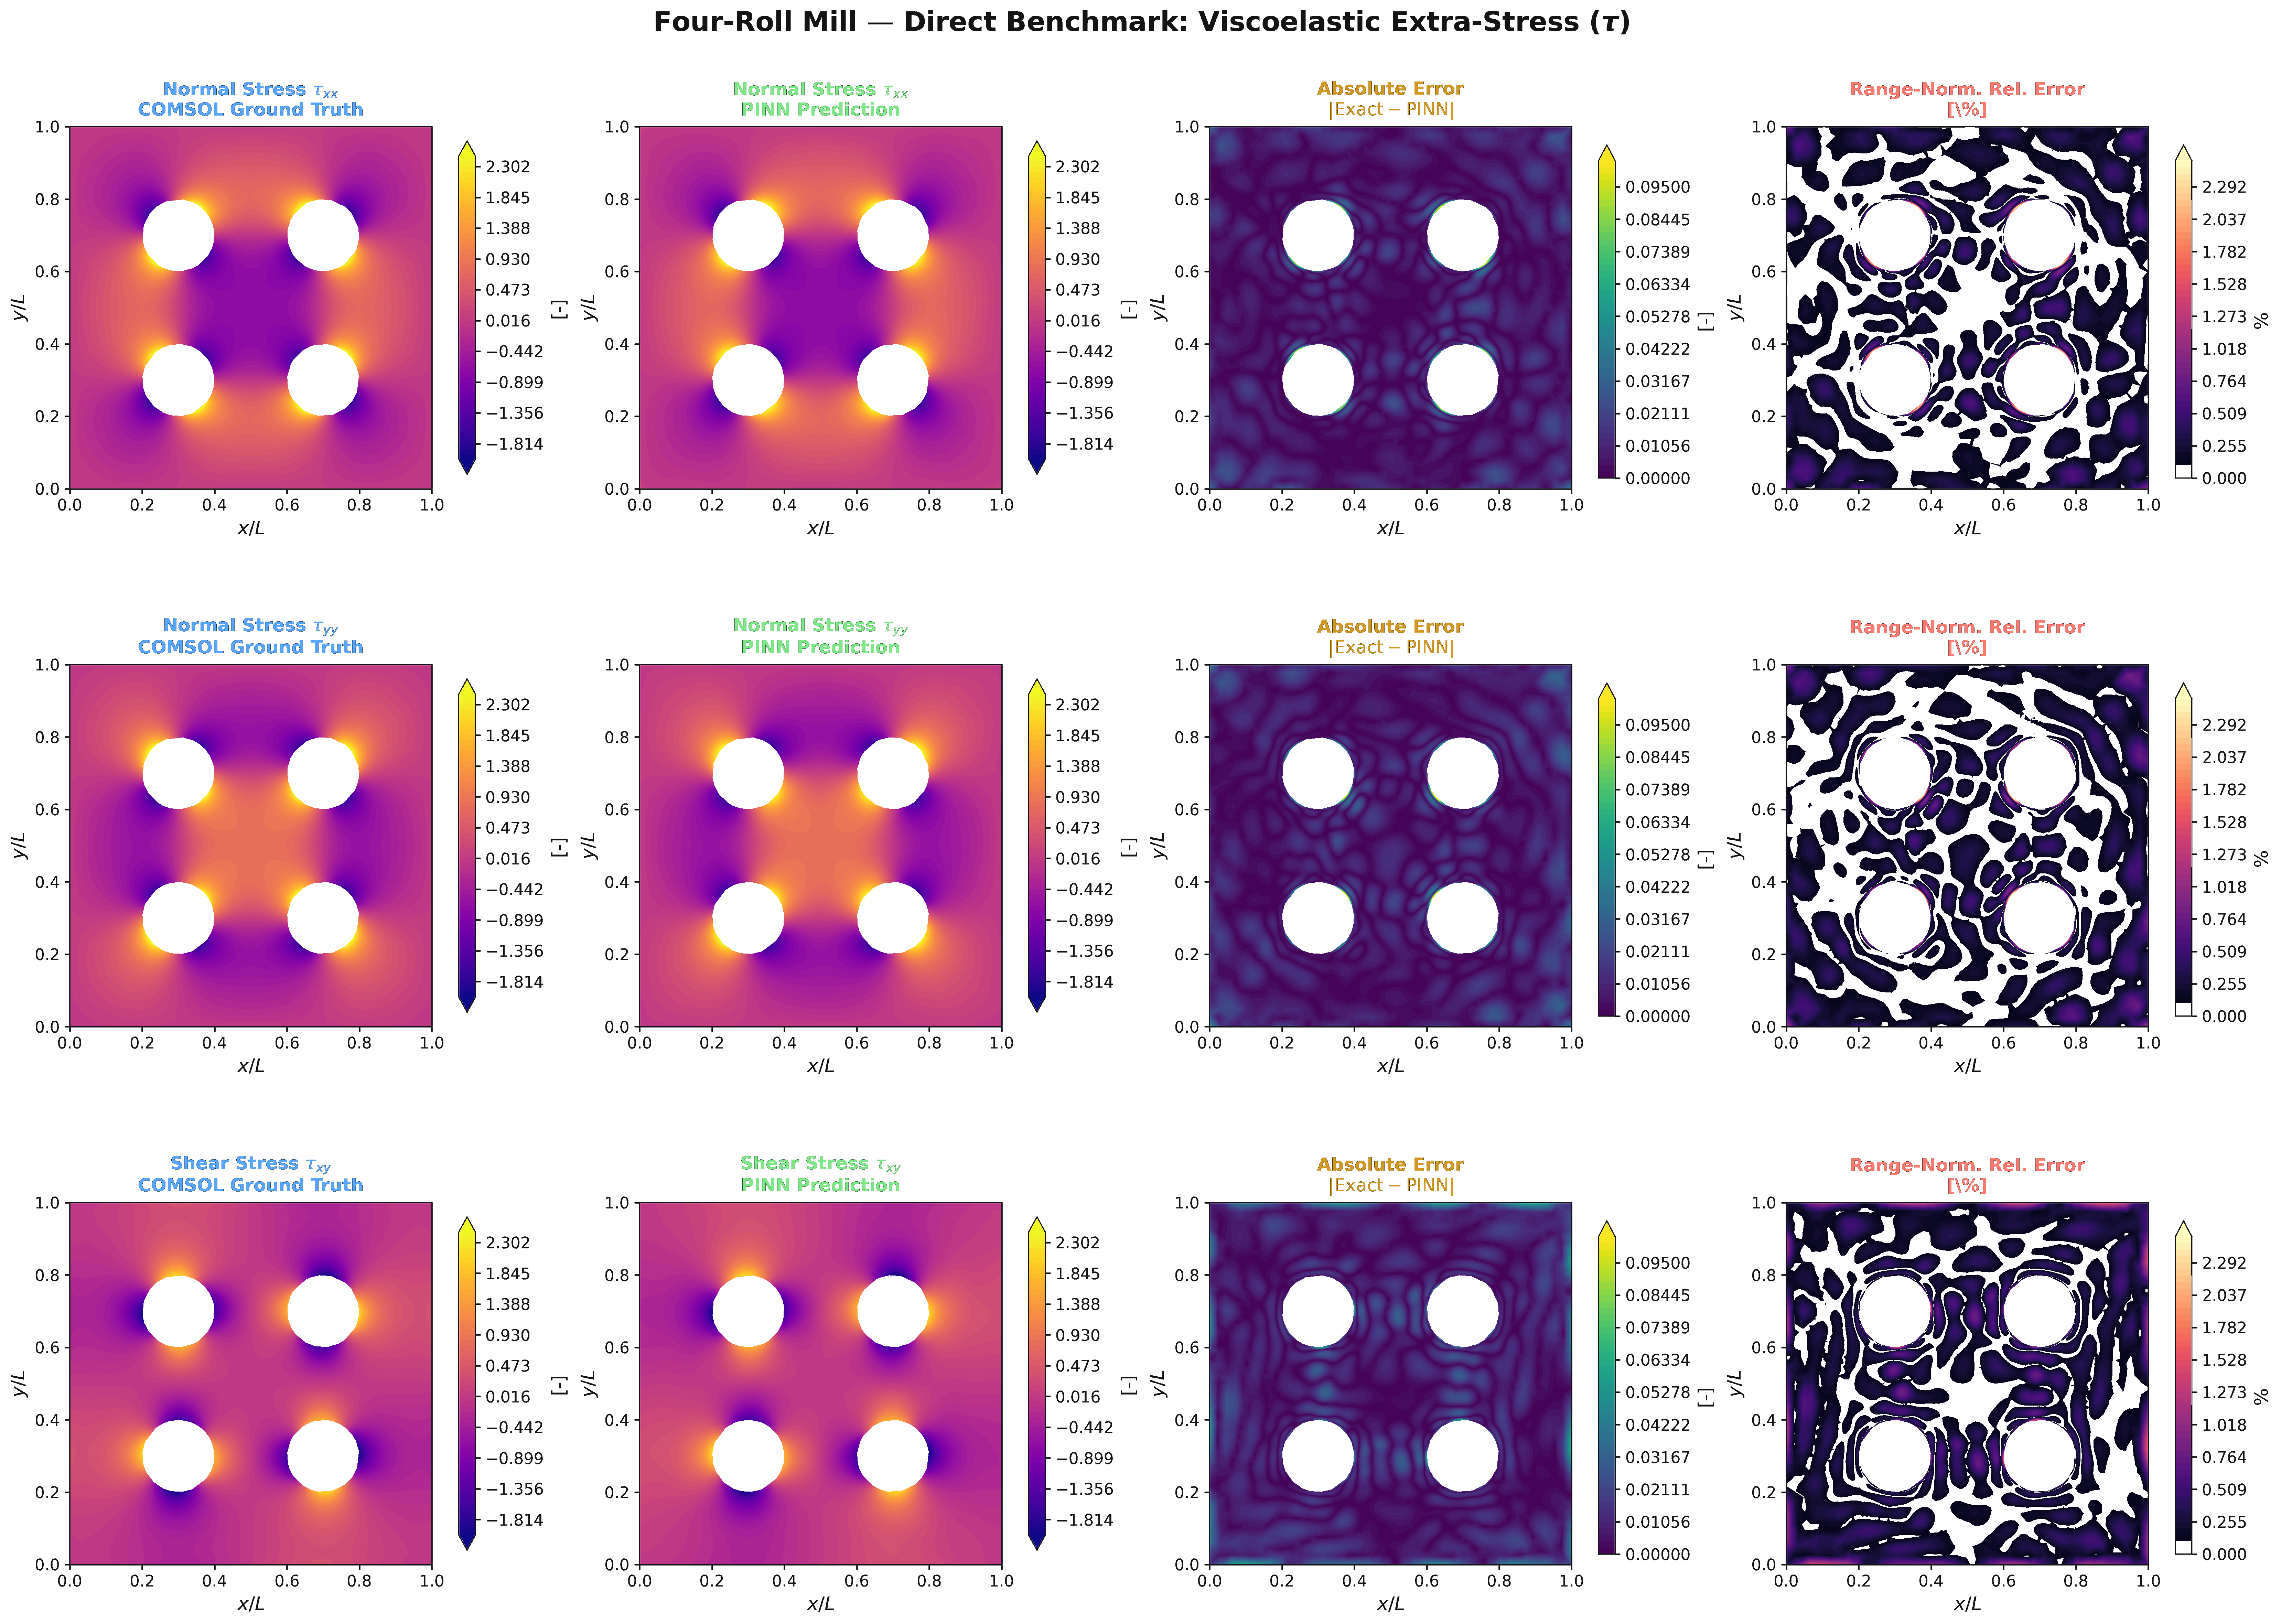
\includegraphics[width=\linewidth]{media/fig3_diretto_stress.png}
    \caption{Direct problem viscoelastic extra-stress tensor validation: COMSOL ground truth, PINN predictions, and absolute errors for normal components $(\tau_{xx}, \tau_{yy})$ and shear component $\tau_{xy}$.}
    \label{fig:direct_stress}
\end{figure}

\subsection{Hydrodynamic Pressure Recovery and Gauge Calibration}
In incompressible fluid mechanics, absolute pressure $p$ is determined only up to an arbitrary hydrostatic constant $C$.
This occurs because pressure enters the governing momentum equations solely through its spatial gradient $\nabla p$.
In discrete numerical simulations, different solvers adopt different reference datum offsets:
COMSOL sets an arbitrary boundary or average gauge,
whereas the PINN is pinned at a discrete coordinate $\boldsymbol{x}_0$.
Consequently, comparing raw PINN predictions directly with COMSOL data yields an apparently large discrepancy ($47.4\%$).
This offset reflects purely a uniform vertical shift rather than an error in flow physics.

To evaluate genuine physical agreement, we calibrate the pressure field
by subtracting the domain mean discrepancy:
\begin{equation}
    p_{\mathrm{cal}}(\boldsymbol{x}) = \hat{p}(\boldsymbol{x}) - \frac{1}{|\Omega|} \int_{\Omega} \left( \hat{p}(\boldsymbol{x}) - p^{\mathrm{ref}}(\boldsymbol{x}) \right) \mathrm{d}\Omega .
    \label{eq:pressure_calibration}
\end{equation}
Equation~\eqref{eq:pressure_calibration} aligns the hydrostatic reference levels of both fields
without altering the spatial gradient: $\nabla p_{\mathrm{cal}} \equiv \nabla \hat{p}$.
As shown in Figure~\ref{fig:direct_pressure},
the calibrated pressure field exhibits close physical agreement with COMSOL ($L_2$ error of $3.42\%$).
This confirms that the reconstructed pressure gradient balances viscous dissipation and polymeric stress divergence
across all 125{,}456 mesh nodes.

\begin{figure}[htbp]
    \centering
    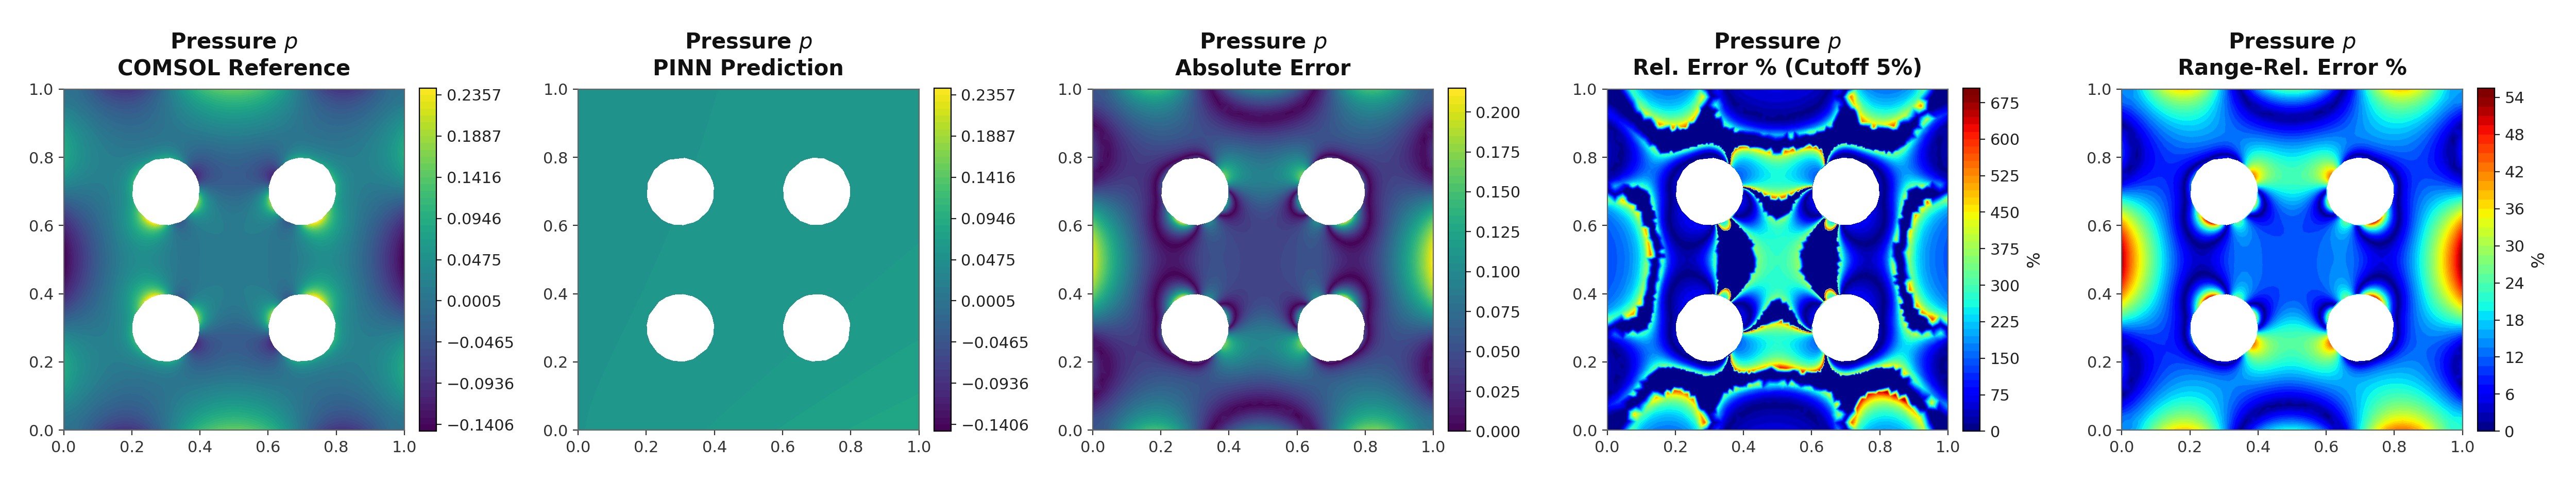
\includegraphics[width=\linewidth]{media/fig2_diretto_pressione.png}
    \caption{Hydrodynamic pressure field reconstruction: COMSOL ground truth, raw and gauge-calibrated PINN predictions, and spatial error distributions, demonstrating close agreement with reference pressure gradients ($L_2$ error of $3.42\%$ upon hydrostatic offset calibration).}
    \label{fig:direct_pressure}
\end{figure}

% ============================================================
% 4.4 INVERSE PROBLEM: PARAMETER DISCOVERY BENCHMARKS
% ============================================================
\section{Inverse Problem: Rheological Parameter Discovery Benchmarks}
\label{sec:inverse_parameter_discovery}

In inverse discovery mode, the PINN operates as a "virtual rheometer":
\textit{we supply no internal stress measurements to the network}.
The model assimilates kinematic velocity data across the domain (representing planar PIV measurements),
kinematic boundary conditions on solid surfaces,
and the auxiliary wall-stress anchor on rotating cylinders ($\mathcal{L}_{\mathrm{roll\_stress}}$).
Crucially, internal polymeric extra-stresses $(\tau_{xx}, \tau_{xy}, \tau_{yy})$ and hydrodynamic pressure $p$
remain entirely latent and unobserved.
They are inferred simultaneously alongside governing fluid parameters via PDE residual minimization.

\subsection{The Four Canonical Benchmarks}
We evaluate four challenging inverse benchmarks spanning linear and non-linear constitutive regimes:
\begin{itemize}
    \item \textbf{Benchmark 1 (Canonical Oldroyd-B from Scratch)}:
    Modest elasticity ($Wi = 0.08$), trained ex-novo for 50{,}000 iterations.
    \item \textbf{Benchmark 2 (High-Elasticity Oldroyd-B via Transfer Learning)}:
    Elevated elasticity ($Wi = 1.17$, $\lambda = 0.70\,\mathrm{s}$),
    initialized using weights from a lower-$Wi$ checkpoint and fine-tuned for 25{,}000 iterations.
    \item \textbf{Benchmark 3 (Non-linear Giesekus with Blind Guess from Scratch)}:
    Fluid with non-linear mobility ($\alpha^{\mathrm{true}} = 0.35$),
    initialized with a blind guess $\alpha_0 = 0.25$ and trained for 50{,}000 iterations.
    \item \textbf{Benchmark 4 (Extreme-Mobility Giesekus via Transfer Learning)}:
    Maximum physical mobility ($\alpha^{\mathrm{true}} = 0.50$, $\lambda = 0.30\,\mathrm{s}$, $\mu_p = 0.05\,\mathrm{Pa\cdot s}$),
    fine-tuned via Transfer Learning for 25{,}000 iterations.
\end{itemize}
These four benchmarks cover both linear Hookean and non-linear shear-thinning response
over relaxation times ranging from $0.05\,\mathrm{s}$ to $0.70\,\mathrm{s}$.

Table~\ref{tab:inverse_benchmarks} summarizes parameter estimation accuracy and kinematic errors across these benchmarks.

\begin{table}[htbp]
    \centering
    \small
    \caption{Inverse parameter discovery results across the four representative benchmarks on the M125k grid.}
    \label{tab:inverse_benchmarks}
    \resizebox{\textwidth}{!}{%
    \begin{tabular}{cllcccc}
        \hline
        \textbf{\#} & \textbf{Model} & \textbf{Strategy} & \textbf{Target Parameter} & \textbf{PINN Estimation} & \textbf{Error} & \textbf{$L_2(u,v)$} \\
        \hline
        \textbf{1} & \textbf{Oldroyd-B} & Ex-Novo & $\lambda = 0.050\,\mathrm{s}$ & $\mathbf{0.0502\,\mathrm{s}}$ & $\mathbf{+0.41\%}$ & \multirow{2}{*}{$0.04\%$} \\
        & ($Wi = 0.08$) & (50k iters) & $\mu_p = 0.900\,\mathrm{Pa\cdot s}$ & $\mathbf{0.9049\,\mathrm{Pa\cdot s}}$ & $\mathbf{+0.54\%}$ & \\
        \hline
        \textbf{2} & \textbf{Oldroyd-B} & Transfer Learning & $\lambda = 0.700\,\mathrm{s}$ & $\mathbf{0.7089\,\mathrm{s}}$ & $\mathbf{+1.27\%}$ & \multirow{2}{*}{$0.33\%$} \\
        & ($Wi = 1.17$) & (25k iters, $-50\%$) & $\mu_p = 0.500\,\mathrm{Pa\cdot s}$ & $\mathbf{0.5019\,\mathrm{Pa\cdot s}}$ & $\mathbf{+0.38\%}$ & \\
        \hline
        \textbf{3} & \textbf{Giesekus} & Ex-Novo (Blind) & $\alpha = 0.350$ & $\mathbf{0.3298}$ & $\mathbf{-5.76\%}$ & \multirow{3}{*}{$0.46\%$} \\
        & ($\alpha_0 = 0.25$) & (50k iters) & $\lambda = 0.100\,\mathrm{s}$ & $\mathbf{0.1032\,\mathrm{s}}$ & $\mathbf{+3.16\%}$ & \\
        & & & $\mu_p = 0.500\,\mathrm{Pa\cdot s}$ & $\mathbf{0.5307\,\mathrm{Pa\cdot s}}$ & $\mathbf{+6.14\%}$ & \\
        \hline
        \textbf{4} & \textbf{Giesekus} & Transfer Learning & $\alpha = 0.500$ & $\mathbf{0.4665}$ & $\mathbf{-6.70\%}$ & \multirow{3}{*}{$0.52\%$} \\
        & (Extreme $\alpha$) & (25k iters, $-50\%$) & $\lambda = 0.300\,\mathrm{s}$ & $\mathbf{0.3077\,\mathrm{s}}$ & $\mathbf{+2.57\%}$ & \\
        & & & $\mu_p = 0.050\,\mathrm{Pa\cdot s}$ & $\mathbf{0.0522\,\mathrm{Pa\cdot s}}$ & $\mathbf{+4.40\%}$ & \\
        \hline
    \end{tabular}%
    }
\end{table}

As detailed in Table~\ref{tab:inverse_benchmarks},
parameter estimation errors for the linear Oldroyd-B model remain below $1.3\%$
across both low and high Weissenberg numbers ($Wi = 0.08$ and $Wi = 1.17$).
For the non-linear Giesekus model, the network simultaneously inverts three coupled parameters $(\alpha, \lambda, \mu_p)$.
It identifies mobility $\alpha$ within $6.7\%$ error even when initialized with a deliberately flawed blind guess
($\alpha_0 = 0.25$ vs $\alpha^{\mathrm{true}} = 0.35$).

\subsection{Convergence Trajectories During Optimization}
Figure~\ref{fig:inverse_convergence} displays parameter evolution during the two-tier Adam + L-BFGS training trajectory on the M125k grid.
During the initial Adam phase, parameters rapidly approach the neighborhood of the true physical values.
Upon transitioning to double-precision L-BFGS,
the parameters settle smoothly toward the target values without oscillatory instabilities.

\begin{figure}[htbp]
    \centering
    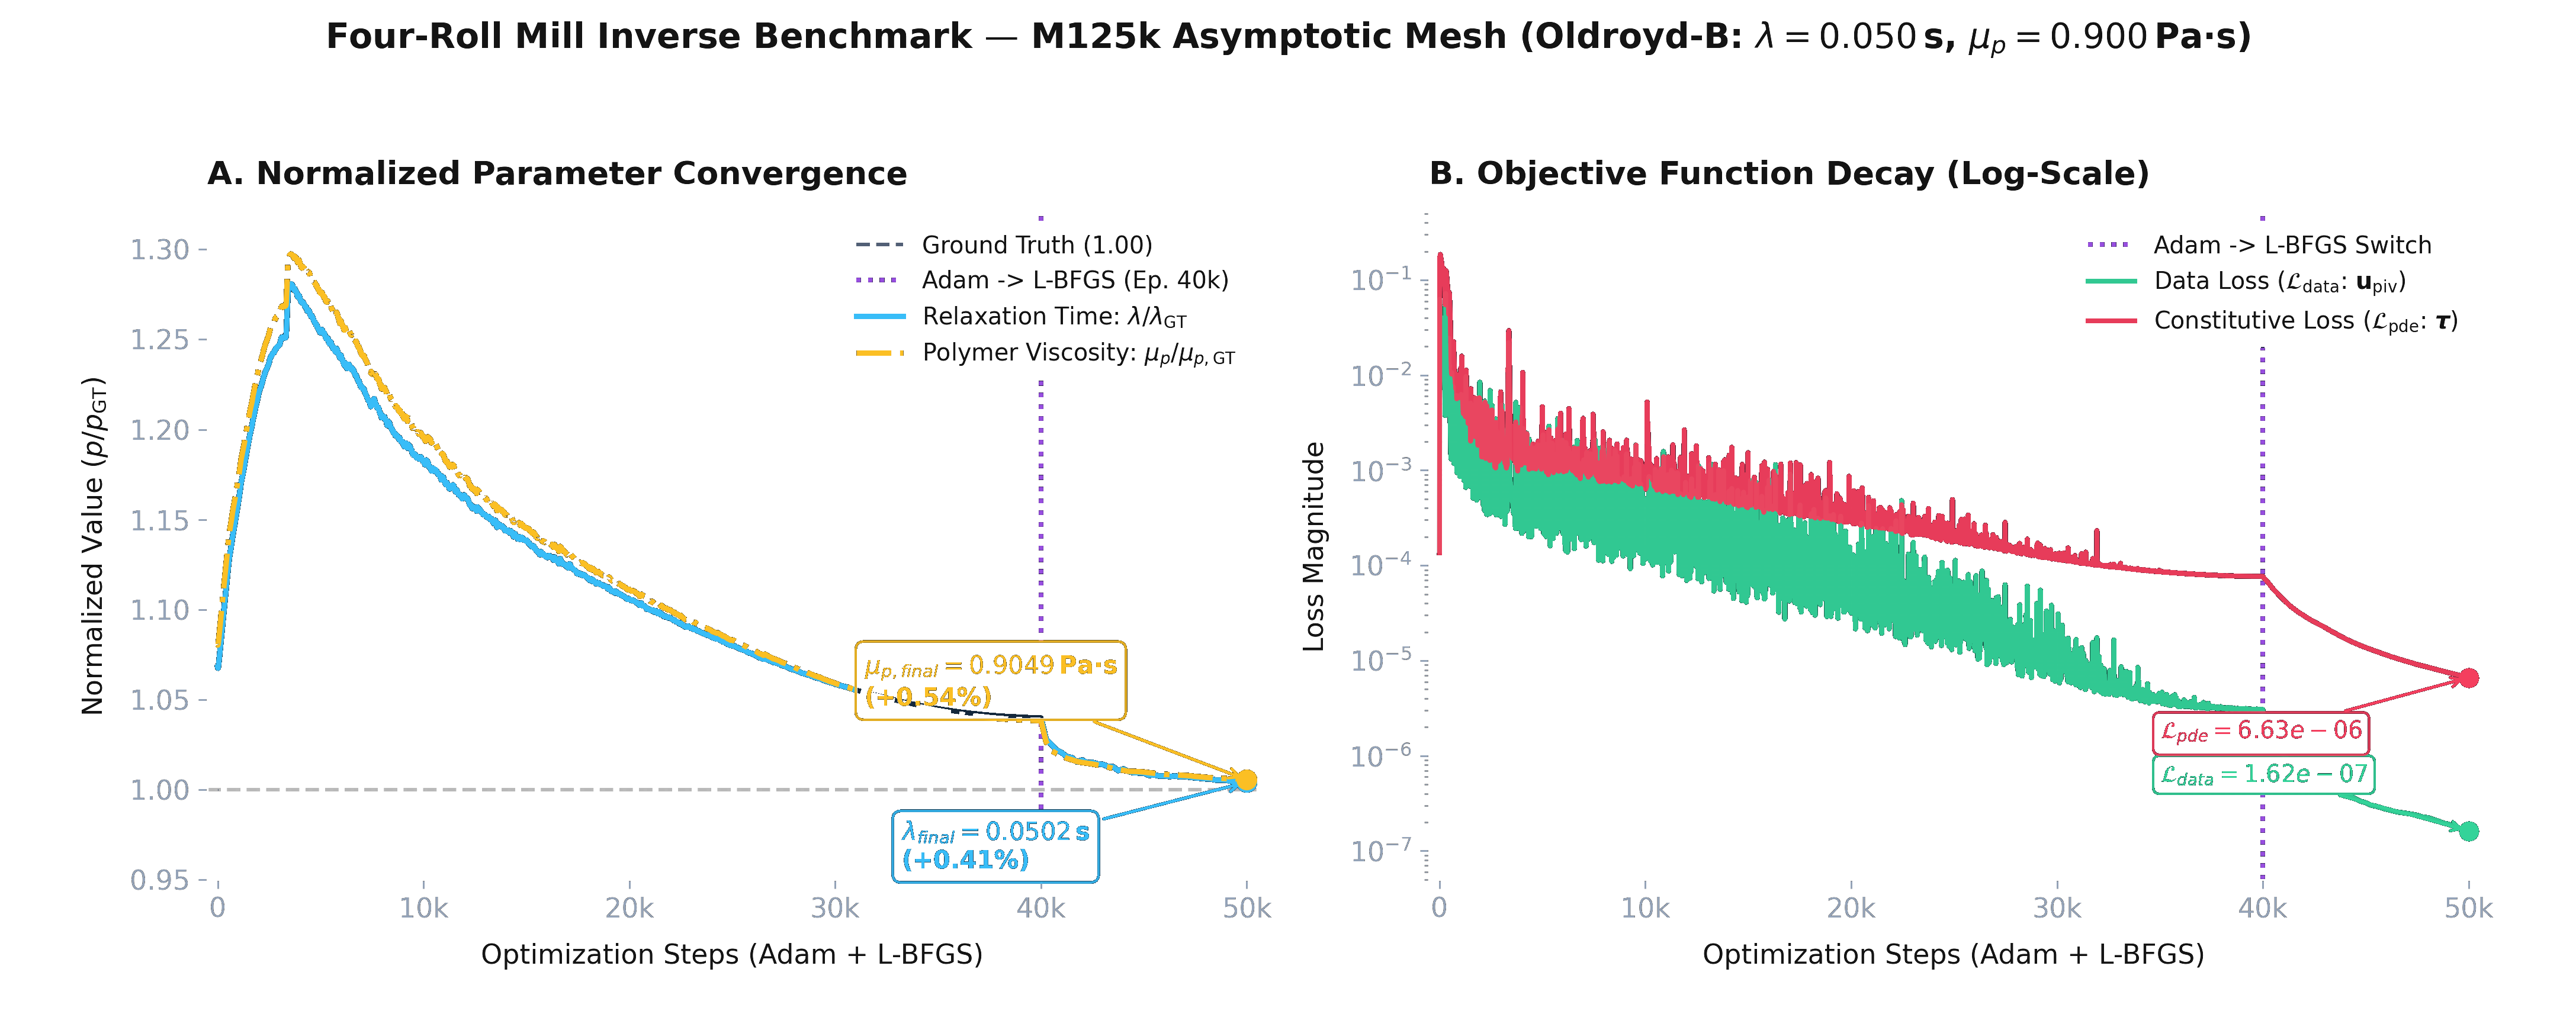
\includegraphics[width=\linewidth]{media/fig4b_inverso_convergence_m125k.png}
    \caption{Parameter convergence trajectories ($\lambda$ and $\mu_p$) during staged Adam (FP32) and L-BFGS (FP64) optimization on the M125k dataset.}
    \label{fig:inverse_convergence}
\end{figure}

% ============================================================
% 4.5 GRID INDEPENDENCE AND COLLOCATION DYNAMICS
% ============================================================
\section{Grid Independence and Collocation Robustness}
\label{sec:grid_independence_collocation}

In classical finite element methods, refining the computational mesh monotonically improves solution accuracy
as interpolation truncation errors diminish.
To examine how collocation density impacts PINN optimization,
we conducted a systematic grid independence study across five mesh resolutions:
5k, 12k, 29k, 52k, and 125k nodes.

\begin{table}[htbp]
    \centering
    \small
    \caption{Collocation density sensitivity and parameter estimation accuracy across five resolutions ($\lambda^{\mathrm{true}} = 0.100\,\mathrm{s}, \mu_p^{\mathrm{true}} = 0.500\,\mathrm{Pa\cdot s}$).}
    \label{tab:grid_independence}
    \resizebox{\textwidth}{!}{%
    \begin{tabular}{lcccccc}
        \hline
        \textbf{Mesh Resolution} & \textbf{Evaluation Nodes} & $\lambda_{\mathrm{est}}$ [s] & $\lambda$ \textbf{Error} & $\mu_{p,\mathrm{est}}$ [Pa·s] & $\mu_p$ \textbf{Error} & \textbf{Velocity $L_2$} \\
        \hline
        \textbf{5k (Coarse)} & \textbf{5{,}086} & $\mathbf{0.1008}$ & $\mathbf{+0.79\%}$ & $\mathbf{0.5103}$ & $\mathbf{+2.06\%}$ & $\mathbf{0.15\%}$ \\
        \textbf{12k} & 12{,}760 & $0.1071$ & $+7.10\%$ & $0.5389$ & $+7.78\%$ & $0.55\%$ \\
        \textbf{29k} & 29{,}392 & $0.1088$ & $+8.79\%$ & $0.5455$ & $+9.10\%$ & $0.58\%$ \\
        \textbf{52k} & 52{,}648 & $0.1062$ & $+6.18\%$ & $0.5323$ & $+6.46\%$ & $0.44\%$ \\
        \textbf{125k (Dense)} & 125{,}456 & $0.1083$ & $+8.32\%$ & $0.5412$ & $+8.24\%$ & $0.50\%$ \\
        \hline
    \end{tabular}%
    }
\end{table}

\begin{figure}[htbp]
    \centering
    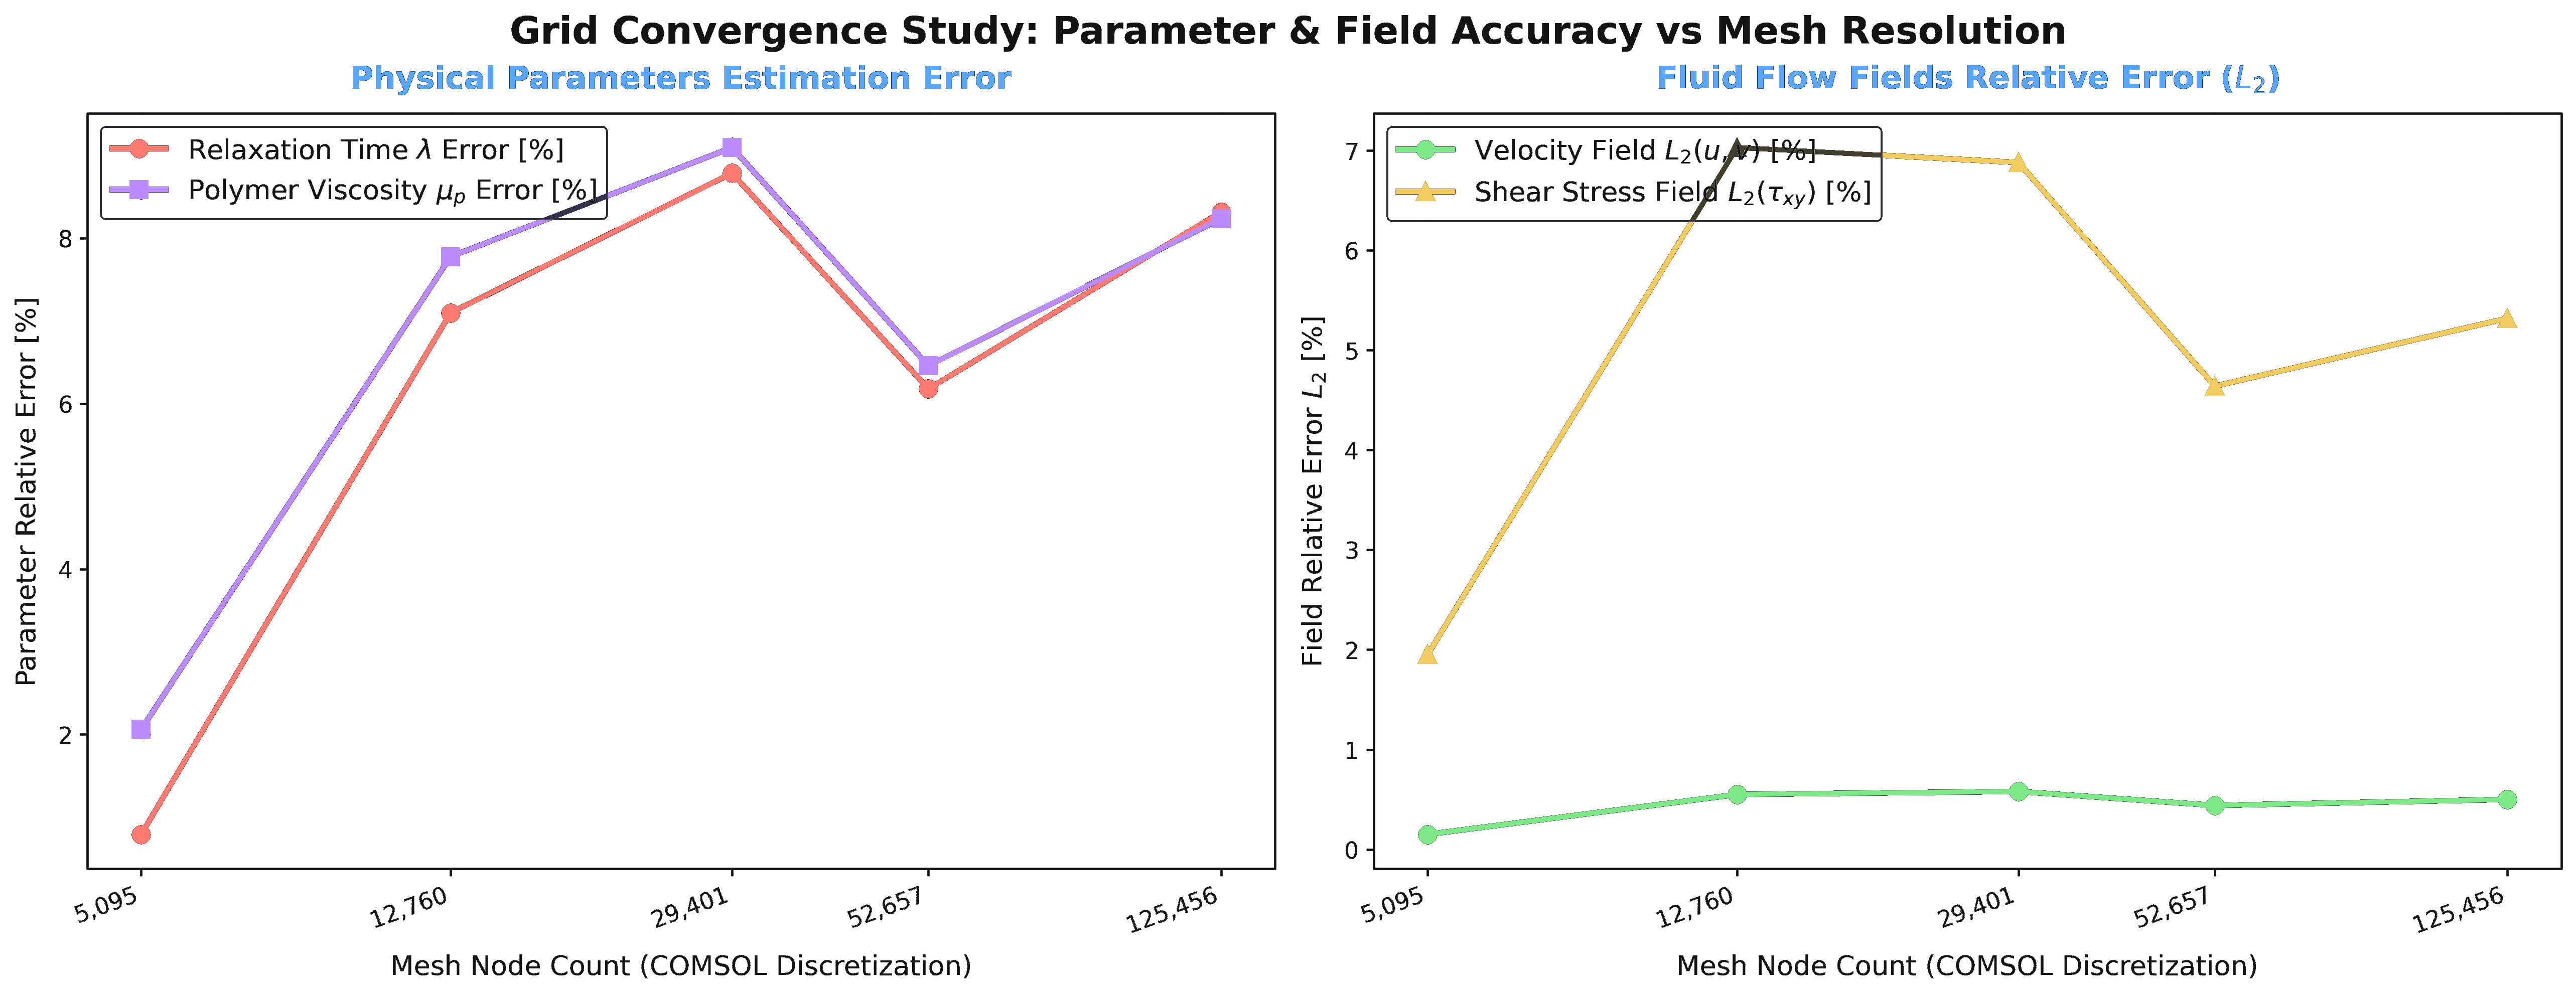
\includegraphics[width=\linewidth]{media/fig5_inverso_mesh_independence.png}
    \caption{Collocation density study: comparison of parameter estimation errors ($\lambda$ and $\mu_p$) and velocity $L_2$ errors across resolutions from 5{,}086 to 125{,}456 collocation points.}
    \label{fig:inverse_mesh_convergence}
\end{figure}

As presented in Table~\ref{tab:grid_independence} and visualized in Figure~\ref{fig:inverse_mesh_convergence},
parameter estimation errors remain confined within a single-digit band (between $0.8\%$ and $8.8\%$)
across a 25-fold increase in collocation density.
Interestingly, accuracy does not improve monotonically with increasing point density:
the coarse 5k dataset ($5{,}086$ points) achieves the lowest estimation error ($+0.79\%$ on $\lambda$, $+2.06\%$ on $\mu_p$),
while denser sets stabilize around $6\text{--}8\%$ error. 

Rather than implying an intrinsic superiority of sparser grids,
this non-monotonic behavior can be understood through network capacity and optimization dynamics.
Our deep architecture possesses a fixed parameter budget (approximately $1.5 \times 10^5$ trainable weights across the three heads).
Beyond a certain collocation threshold, adding further spatial points does not monotonically enhance resolution
because the representation capacity of the network saturates.
Furthermore, in high-density datasets, localized gradient norms in roller boundary layers can alter the balance of the composite loss.
Crucially, the solver demonstrates robustness across the investigated sampling range:
even with coarse collocation, the network recovers the rheological parameters
and resolves the four-roll mill kinematics with high fidelity ($L_2(u,v) \le 0.58\%$).

% ============================================================
% 4.6 TRANSFER LEARNING EFFICIENCY AND STABILITY
% ============================================================
\section{Transfer Learning Efficiency and Numerical Stability}
\label{sec:transfer_learning_analysis}

Training viscoelastic PINNs from scratch for each operating condition is computationally demanding
(requiring approximately 50{,}000 iterations per run).
Moreover, it risks convergence toward suboptimal local minima at elevated Weissenberg numbers. 

To overcome these hurdles, we implemented a Transfer Learning (TL) pipeline:
\begin{enumerate}
    \item \textbf{Base Model Pre-training}:
    We pre-train the network on a moderate baseline case (e.g., Oldroyd-B at $\lambda = 0.05\,\mathrm{s}, Wi = 0.08$).
    \item \textbf{Weight Transfer and Fine-Tuning}:
    We transfer the pre-trained weights as initial conditions for target simulations characterized by high elasticity
    ($\lambda = 0.70\,\mathrm{s}, Wi = 1.17$) or strong non-linear mobility ($\alpha = 0.50$).
\end{enumerate}

The advantages of this workflow are two-fold:
\begin{itemize}
    \item \textbf{50\% Reduction in Optimization Epochs}:
    Fine-tuning converges in 25{,}000 iterations (compared to 50{,}000 iterations from scratch),
    halving computational training duration.
    \item \textbf{High-Weissenberg Numerical Stability}:
    High-$Wi$ runs initialized from scratch frequently stall in local minima where stress gradients surge.
    Weight transfer initializes the network within a favorable basin of attraction,
    facilitating stable convergence even at $Wi > 1$.
\end{itemize}

% ============================================================
% 4.7 GENERAL PHYSICAL INVARIANT: PRESERVATION OF ELASTIC SHEAR MODULUS
% ============================================================
\section{Consistent Recovery of the Elastic Shear Modulus ($G$)}
\label{sec:elastic_modulus_invariant}

A central physical feature observed across all inverse benchmarks is the
\textbf{consistent recovery of the composite Elastic Shear Modulus} $G$:
\begin{equation}
    G = \frac{\mu_p}{\lambda} .
    \label{eq:elastic_modulus_def}
\end{equation}
In dilute and semi-dilute polymeric systems, kinetic theory identifies $G = n k_B T$
as the macroscopic plateau modulus governing the reversible elastic energy storage capacity of macromolecular conformations.
Dividing the linear constitutive equation by $\lambda$ reveals that $G$ enters directly
as the leading scaling prefactor of the rate-of-strain tensor ($2G \boldsymbol{D}$),
representing the primary mechanical stiffness of the fluid continuum.

\begin{table}[htbp]
    \centering
    \small
    \caption{Identification of the macroscopic elastic shear modulus $G = \mu_p / \lambda$ across inverse benchmarks.}
    \label{tab:elastic_modulus_table}
    \begin{tabular}{lcccc}
        \hline
        \textbf{Benchmark Scenario} & $G^{\mathrm{true}}$ [Pa] & $G_{\mathrm{est}}$ [Pa] & \textbf{Relative Error} & \textbf{Individual Errors} ($\lambda, \mu_p$) \\
        \hline
        \textbf{B1: Oldroyd-B} ($Wi=0.08$) & $18.000$ & $18.026$ & $\mathbf{+0.14\%}$ & $+0.41\%, +0.54\%$ \\
        \textbf{B2: Oldroyd-B} ($Wi=1.17$) & $0.714$ & $0.708$ & $\mathbf{-0.88\%}$ & $+1.27\%, +0.38\%$ \\
        \textbf{B3: Giesekus} ($\alpha=0.35$, blind) & $5.000$ & $5.142$ & $\mathbf{+2.85\%}$ & $+3.16\%, +6.14\%$ \\
        \textbf{B4: Giesekus} ($\alpha=0.50$, extreme) & $0.167$ & $0.170$ & $\mathbf{+1.79\%}$ & $+2.57\%, +4.40\%$ \\
        \textbf{PTT Case 1} ($\lambda=1.0, \varepsilon=0.3$) & $0.500$ & $0.506$ & $\mathbf{+1.19\%}$ & $-57.89\%, -57.44\%$ \\
        \textbf{PTT Case 2} ($\lambda=0.7, \varepsilon=0.5$) & $1.357$ & $1.367$ & $\mathbf{+0.70\%}$ & $-61.43\%, -61.19\%$ \\
        \hline
    \end{tabular}
\end{table}

As detailed in Table~\ref{tab:elastic_modulus_table},
the composite modulus $G_{\mathrm{est}} = \mu_{p,\mathrm{est}} / \lambda_{\mathrm{est}}$
is consistently identified with errors bounded within approximately $3\%$ across all test cases.
For linear Oldroyd-B benchmarks, the error remains below $1\%$,
while for non-linear Giesekus benchmarks it reaches $+2.85\%$ and $+1.79\%$. 

Most remarkably, as highlighted by the PTT benchmark,
even when non-linear parameter degradation causes the individual relaxation time $\lambda$
and viscosity $\mu_p$ to collapse by over $57\text{--}61\%$,
their ratio $G = \mu_p / \lambda$ remains preserved to within $1.2\%$.
We hypothesize that the physics-informed loss landscape is structured such that
the composite modulus $G = \mu_p / \lambda$ directly sets the primary elastic stiffness required to sustain the momentum balance.
Consequently, the optimizer locks onto this macroscopic mechanical ratio with high fidelity,
even when the loss surface becomes flat along the $G$-preserving manifold
and impairs the individual identification of molecular relaxation and dissipative coefficients.

% ============================================================
% 4.8 PHYSICAL IDENTIFIABILITY LIMITS AND THEORETICAL DEGRADATION
% ============================================================
\section{Physical Identifiability Limits and Theoretical Degradation Analysis}
\label{sec:identifiability_limits}

While the PINN framework achieves accurate reconstructions across linear and non-linear regimes,
thorough scientific investigation reveals two physical identifiability boundaries
alongside an operational boundary condition requirement.

\subsection{Phase 2 Solvent Viscosity Invariance in Creeping Flow}
\label{subsec:solvent_viscosity_invariance}
In Phase 2, estimating solvent viscosity $\mu_s$ alongside hydrodynamic pressure $p$
by minimizing momentum residuals reveals an identifiability bottleneck.
In the four-roll mill operating regime, the Reynolds number is very small:
\begin{equation}
    Re = 0.0417 \ll 1 .
\end{equation}
In this creeping Stokes regime, inertial convective terms $\rho (\boldsymbol{u} \cdot \nabla \boldsymbol{u})$ are virtually negligible.
The steady momentum equation reduces to:
\begin{equation}
    -\nabla p + \mu_s \nabla^2 \boldsymbol{u} + \nabla \cdot \boldsymbol{\tau} = \boldsymbol{0} .
\end{equation}
Under fixed boundary velocities, variations in $\mu_s$ produce negligible alterations in the solenoidal velocity kinematics,
shifting instead the scalar pressure gradient $\nabla p$.
Consequently, the sensitivity $\partial \mathcal{L}_{\mathrm{mom}} / \partial \mu_s$ becomes nearly flat,
causing gradient-based optimizers to suffer from parameter stagnation.

\subsection{Theoretical Degradation Hypotheses in PTT Fluids}
\label{subsec:ptt_degeneracy_analysis}
When applying the inverse PINN solver to synthetic data generated from the Phan-Thien--Tanner (PTT) model,
an unexpected parameter degradation occurs.
As reported in Table~\ref{tab:ptt_degeneracy}, the extensibility parameter collapses toward zero ($\varepsilon_{\mathrm{est}} \approx 10^{-4}$),
while relaxation time $\lambda$ and polymeric viscosity $\mu_p$ are underestimated by approximately $58-61\%$.
Despite these parameter discrepancies, the predicted velocity field remains in close agreement with the reference solution,
with relative $L_2$ error below $0.9\%$.

\begin{table}[htbp]
    \centering
    \small
    \caption{PTT inverse problem parameter degradation and kinematic error under boundary supervision.}
    \label{tab:ptt_degeneracy}
    \resizebox{\textwidth}{!}{%
    \begin{tabular}{lcccc}
        \hline
        \textbf{Benchmark Dataset} & $\varepsilon^{\mathrm{true}} \to \varepsilon_{\mathrm{est}}$ \textbf{(Error)} & $\lambda^{\mathrm{true}} \to \lambda_{\mathrm{est}}$ \textbf{(Error)} & $\mu_p^{\mathrm{true}} \to \mu_{p,\mathrm{est}}$ \textbf{(Error)} & \textbf{Velocity $L_2$} \\
        \hline
        PTT ($\lambda=1.0, \varepsilon=0.3$) & $0.300 \to 1.7\times 10^{-4}$ & $1.000 \to 0.421\,\mathrm{s}$ & $0.500 \to 0.213\,\mathrm{Pa\cdot s}$ & \multirow{2}{*}{$\mathbf{0.79\%}$} \\
        \texttt{L1-P0.5-S0.5-A0-E0.3} & ($\mathbf{-99.94\%}$) & ($\mathbf{-57.89\%}$) & ($\mathbf{-57.44\%}$) & \\
        \hline
        PTT ($\lambda=0.7, \varepsilon=0.5$) & $0.500 \to 4.4\times 10^{-4}$ & $0.700 \to 0.270\,\mathrm{s}$ & $0.950 \to 0.369\,\mathrm{Pa\cdot s}$ & \multirow{2}{*}{$\mathbf{0.88\%}$} \\
        \texttt{L0.7-P0.95-S0.05-A0-E0.5} & ($\mathbf{-99.91\%}$) & ($\mathbf{-61.43\%}$) & ($\mathbf{-61.19\%}$) & \\
        \hline
    \end{tabular}%
    }
\end{table}

\begin{figure}[htbp]
    \centering
    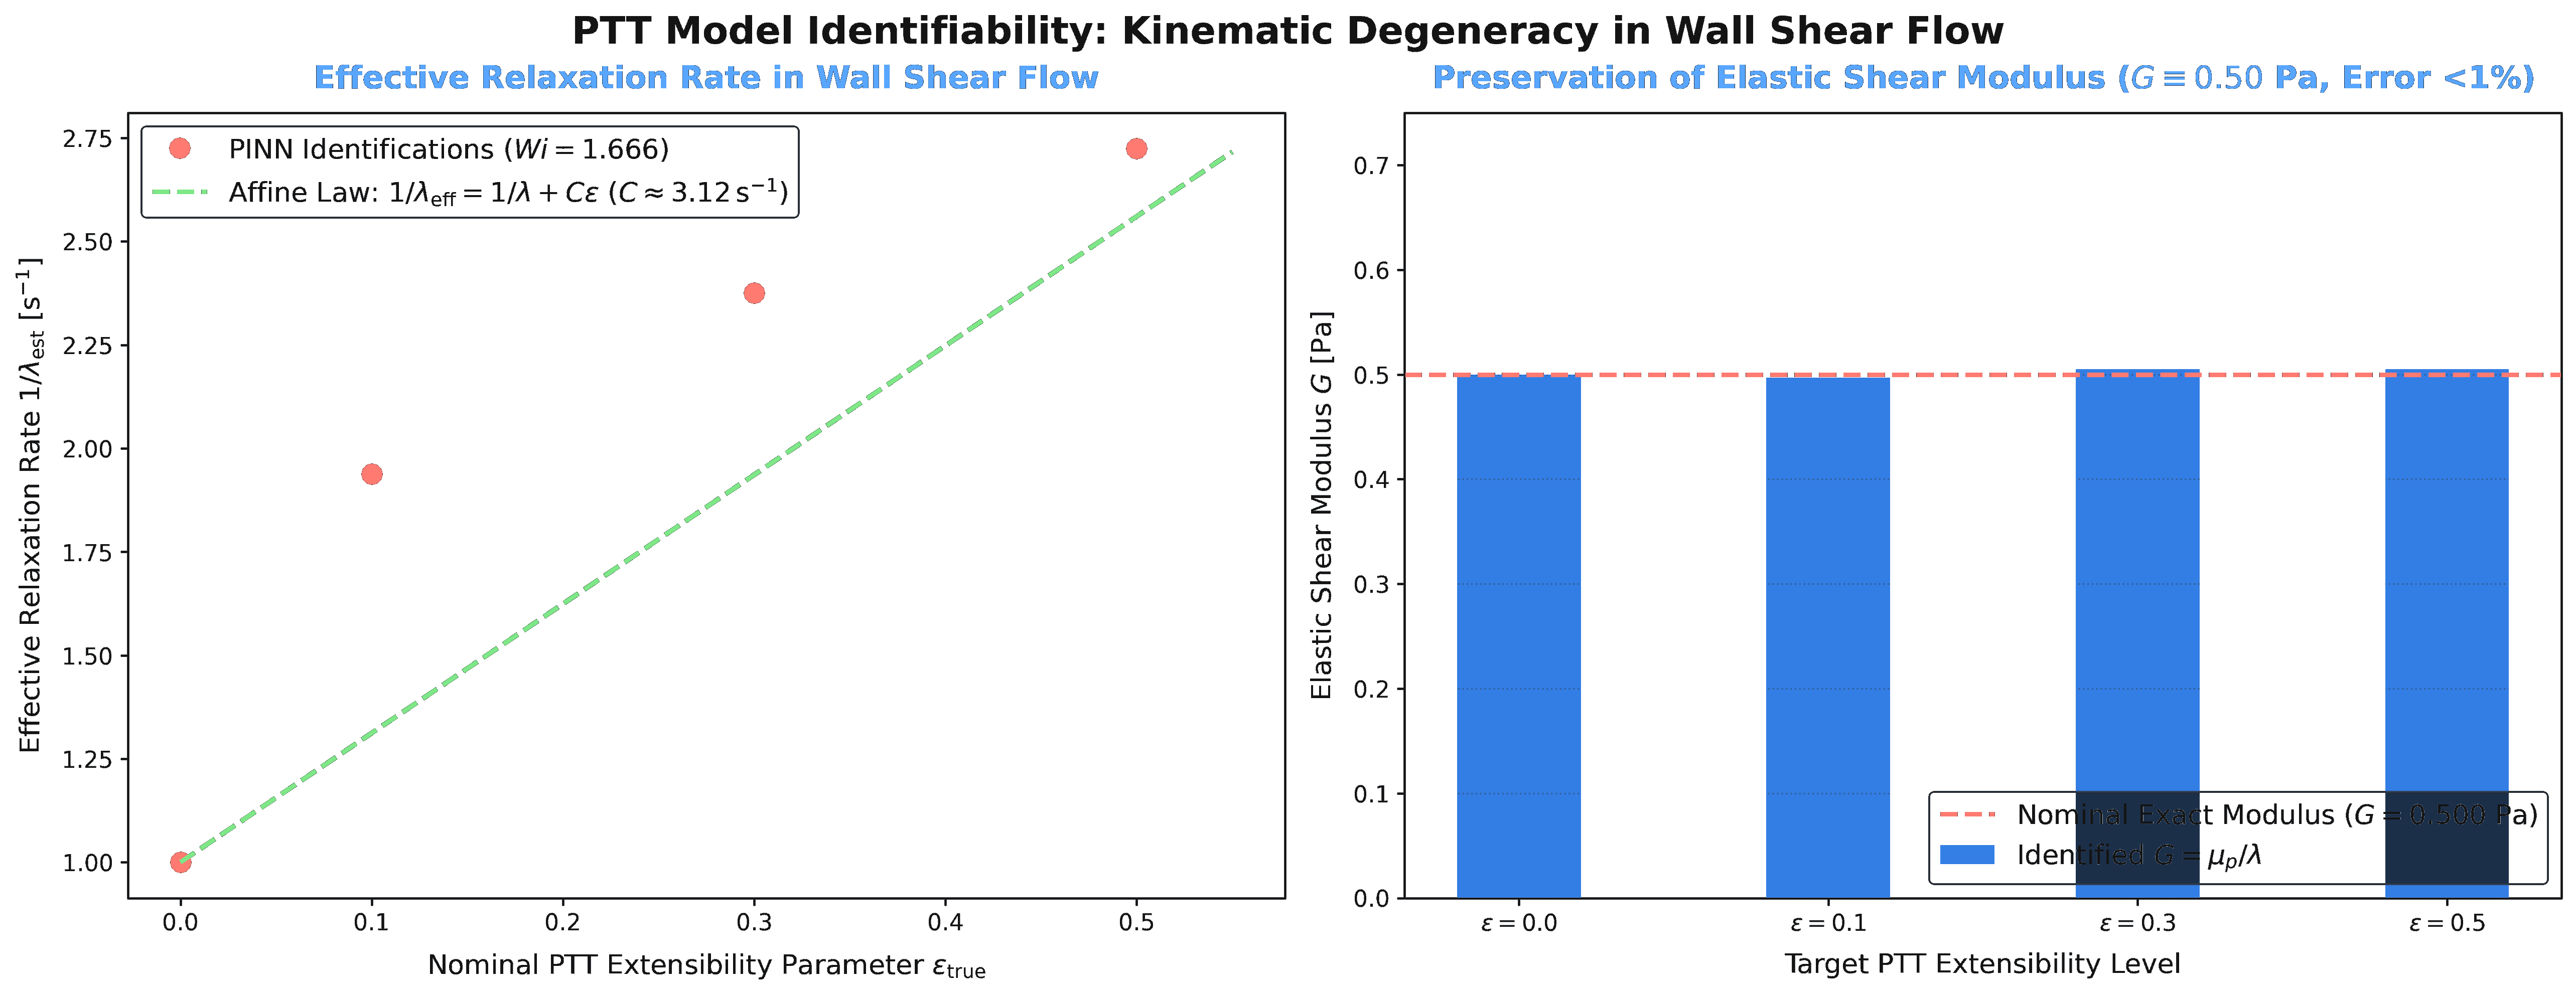
\includegraphics[width=\linewidth]{media/fig6_ptt_degeneracy_insight.png}
    \caption{PTT model identifiability analysis under boundary velocity supervision:
    (left) effective relaxation rate $1/\lambda_{\mathrm{est}}$ as a function of nominal extensibility $\varepsilon_{\mathrm{true}}$ in wall shear flow, compared with the affine shift law ($C \approx 3.12\,\mathrm{s}^{-1}$);
    (right) preservation of the composite elastic shear modulus $G = \mu_p / \lambda = 0.50\,\mathrm{Pa}$ (relative error $< 1\%$) across all tested PTT extensibility levels, demonstrating macroscopic stiffness conservation despite individual parameter degradation.}
    \label{fig:ptt_degeneracy}
\end{figure}

To elucidate the physical origin of this behavior, we propose the following \textit{working theoretical hypotheses}:
\begin{enumerate}
    \item \textbf{Mathematical Consistency of the Differential Operator}:
    Evaluating the PTT constitutive residual offline over the parameter space using the high-fidelity COMSOL ground-truth fields confirms a distinct minimum
    precisely at the true physical parameters ($\lambda = 1.0\,\mathrm{s}, \varepsilon = 0.3$),
    exhibiting a residual loss approximately 25 times lower than that achieved at the network's online attractor.
    This offline diagnostic confirms that the differential residual operator correctly admits the physical parameters as a minimizer.
    This supports our hypothesis that failure during online training stems from the loss landscape conditioning and kinematic degeneracy under boundary supervision,
    rather than an inconsistency in the residual formulation.

    \item \textbf{Wall Shear Flow Degeneracy (Theoretical Working Hypothesis)}:
    In our virtual rheometer setup, velocity supervision is heavily anchored near the rotating cylinder boundaries.
    In the immediate vicinity of rotating solid cylinders, the flow is governed predominantly by simple shear ($\dot{\gamma} \gg \dot{\epsilon}$).
    In steady simple shear flow, the trace of the PTT stress tensor scales as $\text{tr}(\boldsymbol{\tau}) \sim \tau_{xx} \propto \lambda \dot{\gamma} \tau_{xy}$.
    Substituting this scaling into the PTT relaxation function yields an effective linear frequency shift:
    \begin{equation}
        \frac{1}{\lambda_{\mathrm{eff}}} \approx \frac{1}{\lambda_{\mathrm{true}}} + C \cdot \varepsilon_{\mathrm{true}} ,
        \label{eq:ptt_shear_degeneracy}
    \end{equation}
    where $C \approx 3.12\,\mathrm{s}^{-1}$ represents a characteristic shear scaling prefactor related to the wall shear rate in the boundary layer ($\dot{\gamma} \sim U_{\mathrm{roll}} / R$).
    Consequently, an effective linear Oldroyd-B fluid ($\varepsilon = 0, \lambda_{\mathrm{eff}} \approx 0.42\,\mathrm{s}$)
    and a non-linear PTT fluid ($\varepsilon = 0.3, \lambda = 1.0\,\mathrm{s}$) produce virtually indistinguishable kinematic velocity fields
    and wall shear stresses.
    Under velocity-dominated supervision, the optimizer is driven toward the simpler, degenerate Oldroyd-B attractor.
\end{enumerate}

\subsection{Operational Requirement: Physical Necessity of Stress Supervision in Creeping Flow}
\label{subsec:boundary_stress_limitation}
A key operational insight of this work concerns the role of the auxiliary stress supervision term ($\mathcal{L}_{\mathrm{roll\_stress}}$) on the rotating cylinders.
While internal stresses are never supplied to the network,
prescribing boundary stress values on the rollers is physically required in creeping Stokes flow ($Re \ll 1$):
scaling $\mu_s, \mu_p, p$, and $\boldsymbol{\tau}$ by an arbitrary constant leaves the velocity kinematics $\boldsymbol{u}$ unchanged
to within inertial corrections of order $O(Re) \sim 0.04$.
Consequently, purely kinematic velocity data cannot uniquely isolate absolute dimensional viscosities
without a macroscopic stress, torque, or pressure anchoring scale.
In practical experimental applications where direct wall-stress measurements are challenging,
identifying alternative global anchors (such as total motor torque or pressure drop) represents an essential direction for applied viscoelastic PINNs.

% ============================================================
% 4.9 PATHWAYS FORWARD AND COMPUTATIONAL IMPLICATIONS
% ============================================================
\section{Pathways Forward and Computational Engineering Implications}
\label{sec:pathways_forward_implications}

\subsection{Proposals to Overcome Identifiability Boundaries}
Based on the physical degradation mechanisms identified above,
we outline three concrete proposals for future investigations:
\begin{enumerate}
    \item \textbf{Inertial Regime ($Re > 1$)}:
    Operating the four-roll mill at higher Reynolds numbers amplifies the role of inertial convective acceleration $\rho (\boldsymbol{u} \cdot \nabla \boldsymbol{u})$,
    sharpening loss gradients with respect to $\mu_s$ and breaking the creeping Stokes scaling invariance.
    In practice, reaching $Re > 1$ in an experimental four-roll mill with millimeter-scale dimensions
    would require significantly higher roller speeds or lower-viscosity solutions,
    which must be balanced against potential three-dimensional or unsteady flow transitions.
    \item \textbf{Central Stagnation Data Assimilation}:
    Supplementing boundary observations with localized kinematic or birefringence stress measurements around the central extensional stagnation point $(0, 0)$
    would introduce extensional constraints capable of breaking the PTT shear degeneracy.
    \item \textbf{Experimental Noise Assimilation and Asymmetric Roll Kinematics}:
    While prior literature has demonstrated that viscoelastic PINNs can remain stable under synthetic velocity noise up to $10\%$ \cite{thakur2024viscoelasticnet},
    our study focused on deterministic high-fidelity reference data.
    A natural future step is the systematic testing of robustness under simulated experimental measurement noise.
    Furthermore, altering roller angular speed ratios to break four-fold symmetry would enrich the kinematic state space
    and help decouple multi-parameter models.
\end{enumerate}

\subsection{Method Positioning in Computational Fluid Dynamics}
It is essential to clarify the operational role of PINNs within computational fluid dynamics:
\begin{itemize}
    \item PINNs do not aim to replace mature, highly optimized forward CFD solvers
    (such as finite volume or finite element codes) for routine forward flow simulations.
    \item Rather, PINNs act as an \textit{integrative bridge}:
    a mesh-free "virtual rheometer" capable of assimilating kinematic velocity fields
    (such as planar PIV velocity maps) and reconstructing unmeasurable latent physical variables
    (full extra-stress tensors and pressure fields) while discovering the governing constitutive parameters.
\end{itemize}
